\documentclass[notes, aspectratio=1610]{beamer}

% =================================== Colors ================================
\definecolor{base_c}{rgb}{
	0.1411764705882353, 0.6235294117647059, 0.33725490196078434
	}
\definecolor{comp_c}{rgb}{
	0.6235294117647059, 0.1411764705882353, 0.42745098039215684
	}
\definecolor{tri_1}{rgb}{
	0.33725490196078434, 0.1411764705882353, 0.6235294117647059
	}
\definecolor{tri_2}{rgb}{
	0.6235294117647059, 0.33725490196078434, 0.1411764705882353
	}
\definecolor{white}{rgb}{1,1,1}
\usepackage{color, colortbl}

% ================================ Text boxes ==============================
\usepackage[most]{tcolorbox}

% ================================ Symbols ==============================
%\usepackage{bbding}
%\usepackage{pifont}
%\usepackage{wasysym}
%\usepackage{amssymb}

% ========================= Theme =========================================
\usetheme{Berkeley}
\usecolortheme{spruce}
% \setbeamercolor{itemize item}{fg=comp_c,bg=white}
% \setbeamercolor{enumerate item}{fg=comp_c,bg=white}

% ========================= Essential packages ============================
% \usepackage{hyperref}
% \hypersetup{
%     colorlinks = false,
%     linkcolor = comp_c,
%     citecolor = tri_1,
%     filecolor = tri_2,
%     urlcolor = yellow
% }

% ========================= Frame notes systm ============================
%\usepackage{pgfpages}
%\setbeameroption{show notes on second screen}

% ========================= Plotting ======================================
\usepackage{calc}
\usepackage{tikz}
\usetikzlibrary{arrows,
                arrows.meta,
                calc,
		chains,
                quotes,
                positioning,
		shapes,
		topaths,
                shapes.geometric}
\usepackage{graphicx}
\usepackage{graphics}
\usepackage{pgfplots}
\pgfplotsset{width=7cm,compat=1.17}
\usepackage{venndiagram}
% tikz exhibits
\usepackage{tikz}
\usetikzlibrary{shapes,arrows,fit,calc,positioning}
\tikzstyle{box} = [
	draw,
	rectangle,
	rounded corners,
	thick,
	node distance=7em,
	text width=6em,
	text centered,
	minimum height=3.5em
	]
\tikzstyle{container} = [draw, rectangle, dashed, inner sep=2em]
\tikzstyle{lineSq} = [draw, thick, -latex']
\tikzset{
	%Define standard arrow tip
	>=stealth',
	%Define style for boxes
	punkt/.style={
	       rectangle,
	       rounded corners,
	       draw=black, thick,
	       text width=8em,
	       minimum height=3em,
	       text centered},
	punkbig/.style={
		   rectangle,
		   rounded corners,
		   draw=black, thick,
		   text width=5em,
		   minimum height=5em,
		   text centered},
	punkb/.style={
		   rectangle,
		   rounded corners,
		   %draw=black, thick,
		   text width=8em,
		   minimum height=3em,
		   text centered},
	punkc/.style={
	       circle,
	       rounded corners,
	       draw=black, thick,
	       text width=1.5em,
	       minimum height=1.5em,
	       text centered},
	% Define arrow style
	pil/.style={
	       ->,
	       thick,
	       shorten <=2pt,
	       shorten >=2pt,}
}

% ============================= Network viz ===============================
\usepackage{tikz-network}

%% ============================== Tabular =================================
\usepackage{booktabs}
\usepackage{tabularx,ragged2e}
\usepackage{array}
\usepackage{multirow}
\usepackage{siunitx}
  \sisetup{detect-all}
\usepackage{adjustbox}
\usepackage{rotating}
\usepackage{threeparttable}
\usepackage[justification=centering]{caption}

%% ========================== Coding snippets =============================
% Default fixed font does not support bold face
%\usepackage{minted}
%\usemintedstyle{vs}

%% ============================= Math =====================================
\usepackage{mathtools}

% ========================= Infor on authors ==============================
\title[Networks and Value Creation]
{When Do Networks Create Value?}
\subtitle{Bridging Social Capital and Structural Holes}
\author{S.~Santoni\inst{1}\inst{2}}
\institute{
	\inst{1}%
	Bayes Business School
	\and
	\inst{2}%
	Soundcloud
	}
\date{MSc in Business Analytics, 2022/23}

% ========================= TOC  ==========================================
\AtBeginSection[]
{
	\begin{frame}
		       \frametitle{Outline}
		       \tableofcontents[currentsection,currentsubsection]
	\end{frame}
}

% ========================= References ===================================
\usepackage[style=numeric,backend=biber]{biblatex}
\addbibresource{bibliography.bib}

% ========================= Document  ====================================
\begin{document}

\begin{frame}
	\titlepage
\end{frame}

\begin{frame}{Outline}
	\tableofcontents
\end{frame}

% =========================== Session 3 wrapup =============================
\section{Session 3 Wrap Up}

\begin{frame}
	\frametitle{Network Theories across the Various Weeks of SMM638}
	\begin{table}
		\begin{tabular}[c]{l|c|c|c|c|c|c|c|c}
			\textbf{Network theory} & 
			\textbf{2} & 
			\textbf{3} & 
			\textbf{4} & 
			\textbf{5} & 
			\textbf{6} & 
			\textbf{7} & 
			\textbf{9} & 
			\textbf{10}\\
			\hline
			Value creation &  & $\bullet$ & $\bullet$ &  &  &  &  & \\	
			Coordination &  &  &  & $\bullet$ &  &  &  & \\	
			Network change &  &  &  &  & $\bullet$ & $\bullet$ & $\bullet$ & $\bullet$\\	
			Contagion &  &  &  &  &  & $\bullet$ &  & $\bullet$ \\	
		\end{tabular}
	\end{table}
\end{frame}

\begin{frame}
	\frametitle{The Leading Question}
		\begin{center}
			\Large When do networks create value?
		\end{center}
\end{frame}

\begin{frame}
	\frametitle{Groups of Network Theories}
	\centering
	\small
	\begin{table}
		\begin{center}
			\begin{tabular}[c]{l|l|l}
				% \hline
				\textbf{Underlying model} & 
				\textbf{Social capital} &
				\textbf{Social homogeneity}\\
				\hline
				\textbf{Network flow} & \cellcolor{blue!20}{\color{black}{Capitalization (value creation)}} & Contagion  \\
				\hline
				\textbf{Network architecture} & Coordination & Adaptation  (network change)\\
				% \hline
			\end{tabular}
		\end{center}
	\end{table}

	\vspace{1em}

	\raggedright \small Source is~\cite[][page 47]{scott2011}
\end{frame}

\begin{frame}{Theories on Networks and Value Creation}
\begin{columns}
	\begin{column}{0.5\textwidth}
	Mainly, the various theories on the influence of networks on value 
	creation can be grouped into two categories:

	\vspace{1em}

	\begin{itemize}
		\item \textbf{Bridging} social capital theories, whose key 
		      tenet is that sparse networks bring value to 
		      individuals and groups by facilitating fresh courses 
		      of action and new ideas --- a process called 
		      \textbf{network brokerage} 
		\item \textbf{Bonding} social capital theories, whose key 
		      tenet is that dense networks bring value to 
		      individuals and groups by fostering cooperation and trust
		      ---  a process called \textbf{network closure}
	\end{itemize}
	\end{column}
	\begin{column}{0.5\textwidth}
		\centering
		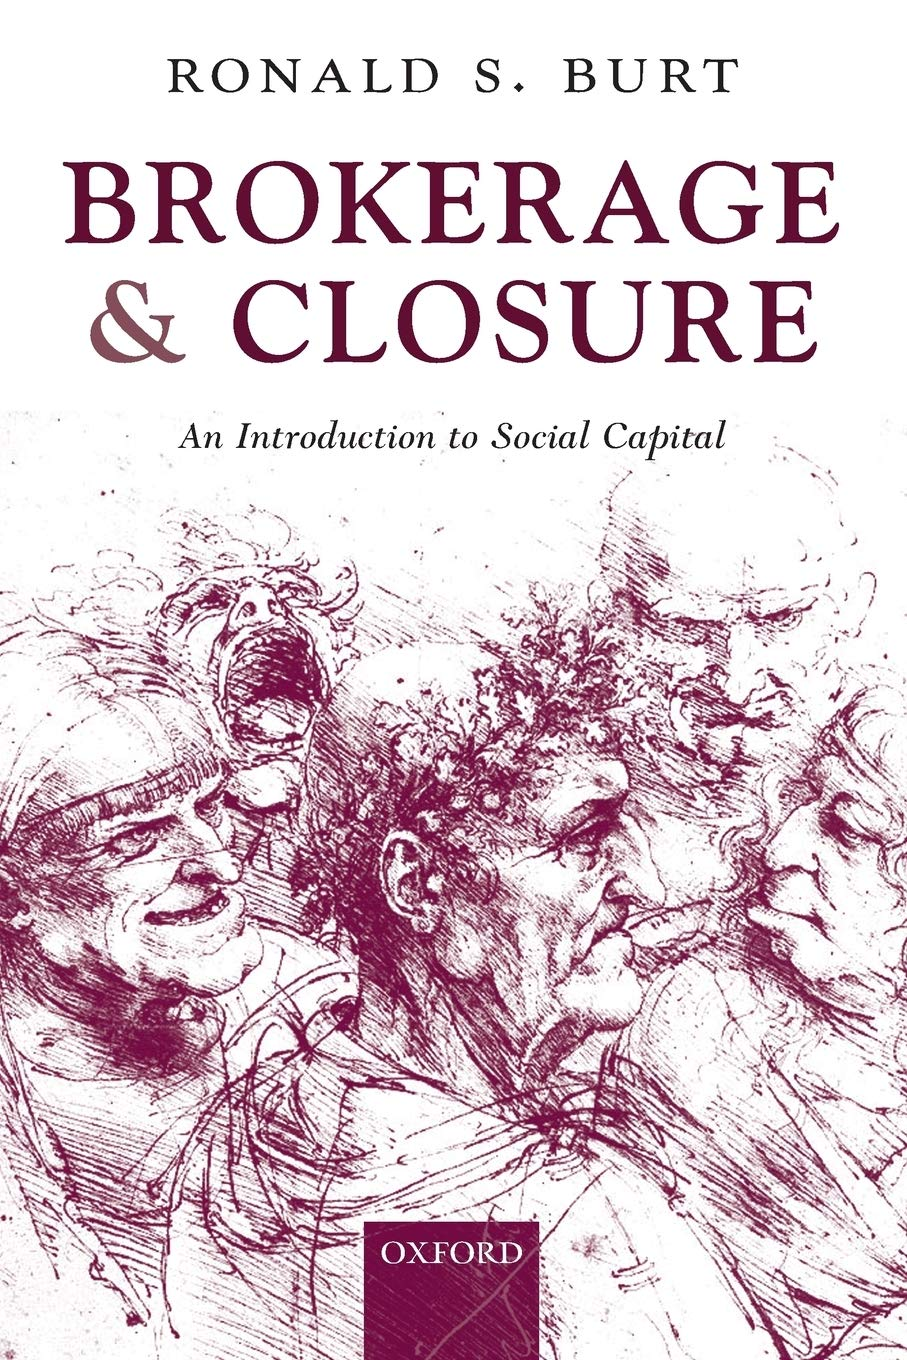
\includegraphics[width=0.75\textwidth]{images/brokerage_and_closure.jpeg}
	\end{column}
\end{columns}
\end{frame}

\begin{frame}{What Is the Outcome of Dense Networks?}
	\begin{figure}
		\resizebox{0.85\textwidth}{!}{
		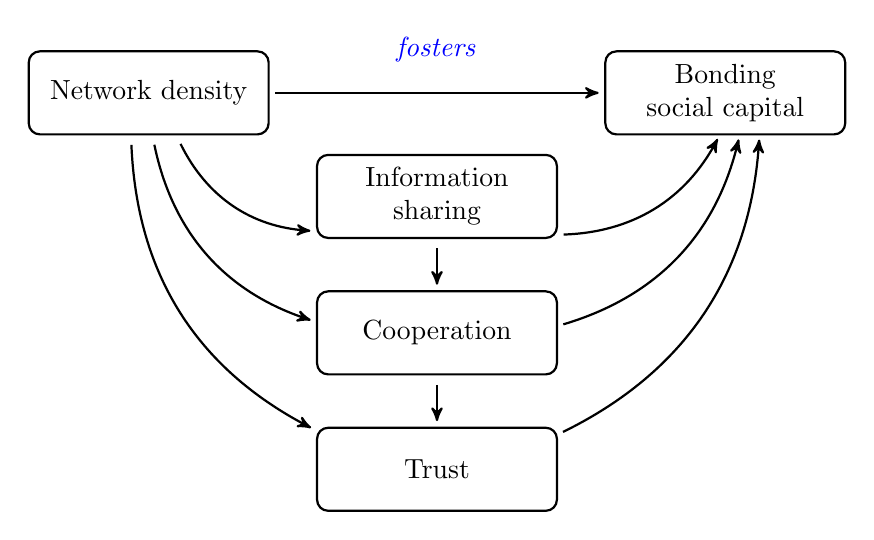
\begin{tikzpicture}[node distance=1cm, auto,] % no additional information
		\node[](d){};
		\node[punkt,left=2cm of d](dn){Network density};
		\node[punkt, label={[align=right]}, right=2cm of d](bsc){Bonding\\social capital}
		edge[pil, <-, bend left=0](dn.east);
		\node[above=0.15cm of d](edge_label){\textcolor{blue}{\textit{fosters}}};
		\node[below=0.15cm of d](d0){};
		\node[right=3.35cm of d0](d1){};
                \node[right=0.001cm of d1](d2){};
		\node[right=0.001cm of d2](d3){};
		\node[below=-0.2cm of dn](d5){};
                \node[right=0.001cm of d5](d4){};
		\node[left=0.001cm of d5](d6){};
		% \pause
		\node[punkt, below=0.65cm of d](info_sharing){Information sharing}
		edge[pil, <-, bend left=30](d4)
		edge[pil, ->, bend right=30] (d1.south);
		% \pause 
		% \pause
		\node[punkt, below=0.65cm of info_sharing](cooperation){Cooperation}
		edge[pil, <-, bend left=30](d5)
		edge[pil, ->, bend right=30] (d2.south);
		% \pause
		% \pause
		\node[punkt, below=0.65cm of cooperation](trust){Trust}
		edge[pil, <-, bend left=30](d6)
		edge[pil, ->, bend right=30] (d3.south);
		\node[below=-0.2cm of cooperation](cooperation_1){}
		edge[pil, ->](trust.north);
		\node[below=-0.2cm of info_sharing](info_sharing_1){}
		edge[pil, ->](cooperation.north);
	\end{tikzpicture}}
\end{figure}
\end{frame}

\begin{frame}{Density Metrics}
	\begin{tcolorbox}[
		colback=comp_c!5!white,
		colframe=comp_c!90!black,
		title={\centering !! Pay attention !!}]
		There is no single metric capturing the concept of network density
	\end{tcolorbox}

	\vspace{2em}

	In practice, we use complementary metrics such as 

	\begin{itemize}
		\item Average degree 
		\item Degree distribution 
		\item Connectdeness
		\item Clustering coefficient
	\end{itemize}
\end{frame}

\begin{frame}{Average Degree}{}
	\begin{columns}
		\begin{column}{0.33\textwidth}

			'Average Degree' is the mean number of connections 
			per node in a network

			\begin{equation*}
				\langle k \rangle = \frac{1}{N}\sum_{i=1}^{N}k_{i} 
			\end{equation*}
			
		\end{column}
		\begin{column}{0.33\textwidth}
			\centering

			\textbf{A} ---  a `star'
			
			\vspace{1em}

			%% Creator: Matplotlib, PGF backend
%%
%% To include the figure in your LaTeX document, write
%%   \input{<filename>.pgf}
%%
%% Make sure the required packages are loaded in your preamble
%%   \usepackage{pgf}
%%
%% Figures using additional raster images can only be included by \input if
%% they are in the same directory as the main LaTeX file. For loading figures
%% from other directories you can use the `import` package
%%   \usepackage{import}
%%
%% and then include the figures with
%%   \import{<path to file>}{<filename>.pgf}
%%
%% Matplotlib used the following preamble
%%   \usepackage{fontspec}
%%   \setmainfont{DejaVuSerif.ttf}[Path=\detokenize{/Users/sbbk475/opt/anaconda3/envs/tech_sci/lib/python3.9/site-packages/matplotlib/mpl-data/fonts/ttf/}]
%%   \setsansfont{DejaVuSans.ttf}[Path=\detokenize{/Users/sbbk475/opt/anaconda3/envs/tech_sci/lib/python3.9/site-packages/matplotlib/mpl-data/fonts/ttf/}]
%%   \setmonofont{DejaVuSansMono.ttf}[Path=\detokenize{/Users/sbbk475/opt/anaconda3/envs/tech_sci/lib/python3.9/site-packages/matplotlib/mpl-data/fonts/ttf/}]
%%
\begingroup%
\makeatletter%
\begin{pgfpicture}%
\pgfpathrectangle{\pgfpointorigin}{\pgfqpoint{1.550000in}{1.510000in}}%
\pgfusepath{use as bounding box, clip}%
\begin{pgfscope}%
\pgfsetbuttcap%
\pgfsetmiterjoin%
\definecolor{currentfill}{rgb}{1.000000,1.000000,1.000000}%
\pgfsetfillcolor{currentfill}%
\pgfsetlinewidth{0.000000pt}%
\definecolor{currentstroke}{rgb}{1.000000,1.000000,1.000000}%
\pgfsetstrokecolor{currentstroke}%
\pgfsetstrokeopacity{0.000000}%
\pgfsetdash{}{0pt}%
\pgfpathmoveto{\pgfqpoint{0.000000in}{0.000000in}}%
\pgfpathlineto{\pgfqpoint{1.550000in}{0.000000in}}%
\pgfpathlineto{\pgfqpoint{1.550000in}{1.510000in}}%
\pgfpathlineto{\pgfqpoint{0.000000in}{1.510000in}}%
\pgfpathclose%
\pgfusepath{fill}%
\end{pgfscope}%
\begin{pgfscope}%
\pgfpathrectangle{\pgfqpoint{0.000000in}{0.000000in}}{\pgfqpoint{1.550000in}{1.510000in}}%
\pgfusepath{clip}%
\pgfsetbuttcap%
\pgfsetroundjoin%
\pgfsetlinewidth{1.003750pt}%
\definecolor{currentstroke}{rgb}{0.000000,0.000000,0.000000}%
\pgfsetstrokecolor{currentstroke}%
\pgfsetdash{}{0pt}%
\pgfpathmoveto{\pgfqpoint{0.134504in}{0.131033in}}%
\pgfpathlineto{\pgfqpoint{0.775000in}{0.755000in}}%
\pgfusepath{stroke}%
\end{pgfscope}%
\begin{pgfscope}%
\pgfpathrectangle{\pgfqpoint{0.000000in}{0.000000in}}{\pgfqpoint{1.550000in}{1.510000in}}%
\pgfusepath{clip}%
\pgfsetbuttcap%
\pgfsetroundjoin%
\pgfsetlinewidth{1.003750pt}%
\definecolor{currentstroke}{rgb}{0.000000,0.000000,0.000000}%
\pgfsetstrokecolor{currentstroke}%
\pgfsetdash{}{0pt}%
\pgfpathmoveto{\pgfqpoint{0.134504in}{1.378967in}}%
\pgfpathlineto{\pgfqpoint{0.775000in}{0.755000in}}%
\pgfusepath{stroke}%
\end{pgfscope}%
\begin{pgfscope}%
\pgfpathrectangle{\pgfqpoint{0.000000in}{0.000000in}}{\pgfqpoint{1.550000in}{1.510000in}}%
\pgfusepath{clip}%
\pgfsetbuttcap%
\pgfsetroundjoin%
\pgfsetlinewidth{1.003750pt}%
\definecolor{currentstroke}{rgb}{0.000000,0.000000,0.000000}%
\pgfsetstrokecolor{currentstroke}%
\pgfsetdash{}{0pt}%
\pgfpathmoveto{\pgfqpoint{0.775000in}{0.755000in}}%
\pgfpathlineto{\pgfqpoint{1.415496in}{0.131033in}}%
\pgfusepath{stroke}%
\end{pgfscope}%
\begin{pgfscope}%
\pgfpathrectangle{\pgfqpoint{0.000000in}{0.000000in}}{\pgfqpoint{1.550000in}{1.510000in}}%
\pgfusepath{clip}%
\pgfsetbuttcap%
\pgfsetroundjoin%
\pgfsetlinewidth{1.003750pt}%
\definecolor{currentstroke}{rgb}{0.000000,0.000000,0.000000}%
\pgfsetstrokecolor{currentstroke}%
\pgfsetdash{}{0pt}%
\pgfpathmoveto{\pgfqpoint{0.775000in}{0.755000in}}%
\pgfpathlineto{\pgfqpoint{1.415496in}{1.378967in}}%
\pgfusepath{stroke}%
\end{pgfscope}%
\begin{pgfscope}%
\pgfpathrectangle{\pgfqpoint{0.000000in}{0.000000in}}{\pgfqpoint{1.550000in}{1.510000in}}%
\pgfusepath{clip}%
\pgfsetbuttcap%
\pgfsetroundjoin%
\definecolor{currentfill}{rgb}{1.000000,1.000000,1.000000}%
\pgfsetfillcolor{currentfill}%
\pgfsetlinewidth{1.003750pt}%
\definecolor{currentstroke}{rgb}{1.000000,1.000000,1.000000}%
\pgfsetstrokecolor{currentstroke}%
\pgfsetdash{}{0pt}%
\pgfsys@defobject{currentmarker}{\pgfqpoint{-0.120281in}{-0.120281in}}{\pgfqpoint{0.120281in}{0.120281in}}{%
\pgfpathmoveto{\pgfqpoint{0.000000in}{-0.120281in}}%
\pgfpathcurveto{\pgfqpoint{0.031899in}{-0.120281in}}{\pgfqpoint{0.062496in}{-0.107608in}}{\pgfqpoint{0.085052in}{-0.085052in}}%
\pgfpathcurveto{\pgfqpoint{0.107608in}{-0.062496in}}{\pgfqpoint{0.120281in}{-0.031899in}}{\pgfqpoint{0.120281in}{0.000000in}}%
\pgfpathcurveto{\pgfqpoint{0.120281in}{0.031899in}}{\pgfqpoint{0.107608in}{0.062496in}}{\pgfqpoint{0.085052in}{0.085052in}}%
\pgfpathcurveto{\pgfqpoint{0.062496in}{0.107608in}}{\pgfqpoint{0.031899in}{0.120281in}}{\pgfqpoint{0.000000in}{0.120281in}}%
\pgfpathcurveto{\pgfqpoint{-0.031899in}{0.120281in}}{\pgfqpoint{-0.062496in}{0.107608in}}{\pgfqpoint{-0.085052in}{0.085052in}}%
\pgfpathcurveto{\pgfqpoint{-0.107608in}{0.062496in}}{\pgfqpoint{-0.120281in}{0.031899in}}{\pgfqpoint{-0.120281in}{0.000000in}}%
\pgfpathcurveto{\pgfqpoint{-0.120281in}{-0.031899in}}{\pgfqpoint{-0.107608in}{-0.062496in}}{\pgfqpoint{-0.085052in}{-0.085052in}}%
\pgfpathcurveto{\pgfqpoint{-0.062496in}{-0.107608in}}{\pgfqpoint{-0.031899in}{-0.120281in}}{\pgfqpoint{0.000000in}{-0.120281in}}%
\pgfpathclose%
\pgfusepath{stroke,fill}%
}%
\begin{pgfscope}%
\pgfsys@transformshift{0.134504in}{0.131033in}%
\pgfsys@useobject{currentmarker}{}%
\end{pgfscope}%
\begin{pgfscope}%
\pgfsys@transformshift{0.134504in}{1.378967in}%
\pgfsys@useobject{currentmarker}{}%
\end{pgfscope}%
\begin{pgfscope}%
\pgfsys@transformshift{0.775000in}{0.755000in}%
\pgfsys@useobject{currentmarker}{}%
\end{pgfscope}%
\begin{pgfscope}%
\pgfsys@transformshift{1.415496in}{0.131033in}%
\pgfsys@useobject{currentmarker}{}%
\end{pgfscope}%
\begin{pgfscope}%
\pgfsys@transformshift{1.415496in}{1.378967in}%
\pgfsys@useobject{currentmarker}{}%
\end{pgfscope}%
\end{pgfscope}%
\begin{pgfscope}%
\definecolor{textcolor}{rgb}{0.000000,0.000000,0.000000}%
\pgfsetstrokecolor{textcolor}%
\pgfsetfillcolor{textcolor}%
\pgftext[x=0.134504in,y=0.131033in,,]{\color{textcolor}\sffamily\fontsize{12.000000}{14.400000}\selectfont 1}%
\end{pgfscope}%
\begin{pgfscope}%
\definecolor{textcolor}{rgb}{0.000000,0.000000,0.000000}%
\pgfsetstrokecolor{textcolor}%
\pgfsetfillcolor{textcolor}%
\pgftext[x=0.134504in,y=1.378967in,,]{\color{textcolor}\sffamily\fontsize{12.000000}{14.400000}\selectfont 2}%
\end{pgfscope}%
\begin{pgfscope}%
\definecolor{textcolor}{rgb}{0.000000,0.000000,0.000000}%
\pgfsetstrokecolor{textcolor}%
\pgfsetfillcolor{textcolor}%
\pgftext[x=0.775000in,y=0.755000in,,]{\color{textcolor}\sffamily\fontsize{12.000000}{14.400000}\selectfont 3}%
\end{pgfscope}%
\begin{pgfscope}%
\definecolor{textcolor}{rgb}{0.000000,0.000000,0.000000}%
\pgfsetstrokecolor{textcolor}%
\pgfsetfillcolor{textcolor}%
\pgftext[x=1.415496in,y=0.131033in,,]{\color{textcolor}\sffamily\fontsize{12.000000}{14.400000}\selectfont 4}%
\end{pgfscope}%
\begin{pgfscope}%
\definecolor{textcolor}{rgb}{0.000000,0.000000,0.000000}%
\pgfsetstrokecolor{textcolor}%
\pgfsetfillcolor{textcolor}%
\pgftext[x=1.415496in,y=1.378967in,,]{\color{textcolor}\sffamily\fontsize{12.000000}{14.400000}\selectfont 5}%
\end{pgfscope}%
\end{pgfpicture}%
\makeatother%
\endgroup%

			
			\vspace{1em}

			$\langle k \rangle = \frac{4}{5}$

		\end{column}
		\begin{column}{0.33\textwidth}
			\centering 
			\textbf{B} --- a `dense' network			

			\vspace{1em}

			%% Creator: Matplotlib, PGF backend
%%
%% To include the figure in your LaTeX document, write
%%   \input{<filename>.pgf}
%%
%% Make sure the required packages are loaded in your preamble
%%   \usepackage{pgf}
%%
%% Figures using additional raster images can only be included by \input if
%% they are in the same directory as the main LaTeX file. For loading figures
%% from other directories you can use the `import` package
%%   \usepackage{import}
%%
%% and then include the figures with
%%   \import{<path to file>}{<filename>.pgf}
%%
%% Matplotlib used the following preamble
%%   \usepackage{fontspec}
%%   \setmainfont{DejaVuSerif.ttf}[Path=\detokenize{/Users/sbbk475/opt/anaconda3/envs/tech_sci/lib/python3.9/site-packages/matplotlib/mpl-data/fonts/ttf/}]
%%   \setsansfont{DejaVuSans.ttf}[Path=\detokenize{/Users/sbbk475/opt/anaconda3/envs/tech_sci/lib/python3.9/site-packages/matplotlib/mpl-data/fonts/ttf/}]
%%   \setmonofont{DejaVuSansMono.ttf}[Path=\detokenize{/Users/sbbk475/opt/anaconda3/envs/tech_sci/lib/python3.9/site-packages/matplotlib/mpl-data/fonts/ttf/}]
%%
\begingroup%
\makeatletter%
\begin{pgfpicture}%
\pgfpathrectangle{\pgfpointorigin}{\pgfqpoint{1.550000in}{1.510000in}}%
\pgfusepath{use as bounding box, clip}%
\begin{pgfscope}%
\pgfsetbuttcap%
\pgfsetmiterjoin%
\definecolor{currentfill}{rgb}{1.000000,1.000000,1.000000}%
\pgfsetfillcolor{currentfill}%
\pgfsetlinewidth{0.000000pt}%
\definecolor{currentstroke}{rgb}{1.000000,1.000000,1.000000}%
\pgfsetstrokecolor{currentstroke}%
\pgfsetstrokeopacity{0.000000}%
\pgfsetdash{}{0pt}%
\pgfpathmoveto{\pgfqpoint{0.000000in}{0.000000in}}%
\pgfpathlineto{\pgfqpoint{1.550000in}{0.000000in}}%
\pgfpathlineto{\pgfqpoint{1.550000in}{1.510000in}}%
\pgfpathlineto{\pgfqpoint{0.000000in}{1.510000in}}%
\pgfpathclose%
\pgfusepath{fill}%
\end{pgfscope}%
\begin{pgfscope}%
\pgfpathrectangle{\pgfqpoint{0.000000in}{0.000000in}}{\pgfqpoint{1.550000in}{1.510000in}}%
\pgfusepath{clip}%
\pgfsetbuttcap%
\pgfsetroundjoin%
\pgfsetlinewidth{1.003750pt}%
\definecolor{currentstroke}{rgb}{0.000000,0.000000,0.000000}%
\pgfsetstrokecolor{currentstroke}%
\pgfsetdash{}{0pt}%
\pgfpathmoveto{\pgfqpoint{0.134504in}{0.131033in}}%
\pgfpathlineto{\pgfqpoint{0.775000in}{0.755000in}}%
\pgfusepath{stroke}%
\end{pgfscope}%
\begin{pgfscope}%
\pgfpathrectangle{\pgfqpoint{0.000000in}{0.000000in}}{\pgfqpoint{1.550000in}{1.510000in}}%
\pgfusepath{clip}%
\pgfsetbuttcap%
\pgfsetroundjoin%
\pgfsetlinewidth{1.003750pt}%
\definecolor{currentstroke}{rgb}{0.000000,0.000000,0.000000}%
\pgfsetstrokecolor{currentstroke}%
\pgfsetdash{}{0pt}%
\pgfpathmoveto{\pgfqpoint{0.134504in}{0.131033in}}%
\pgfpathlineto{\pgfqpoint{0.134504in}{1.378967in}}%
\pgfusepath{stroke}%
\end{pgfscope}%
\begin{pgfscope}%
\pgfpathrectangle{\pgfqpoint{0.000000in}{0.000000in}}{\pgfqpoint{1.550000in}{1.510000in}}%
\pgfusepath{clip}%
\pgfsetbuttcap%
\pgfsetroundjoin%
\pgfsetlinewidth{1.003750pt}%
\definecolor{currentstroke}{rgb}{0.000000,0.000000,0.000000}%
\pgfsetstrokecolor{currentstroke}%
\pgfsetdash{}{0pt}%
\pgfpathmoveto{\pgfqpoint{0.134504in}{0.131033in}}%
\pgfpathlineto{\pgfqpoint{1.415496in}{0.131033in}}%
\pgfusepath{stroke}%
\end{pgfscope}%
\begin{pgfscope}%
\pgfpathrectangle{\pgfqpoint{0.000000in}{0.000000in}}{\pgfqpoint{1.550000in}{1.510000in}}%
\pgfusepath{clip}%
\pgfsetbuttcap%
\pgfsetroundjoin%
\pgfsetlinewidth{1.003750pt}%
\definecolor{currentstroke}{rgb}{0.000000,0.000000,0.000000}%
\pgfsetstrokecolor{currentstroke}%
\pgfsetdash{}{0pt}%
\pgfpathmoveto{\pgfqpoint{0.134504in}{1.378967in}}%
\pgfpathlineto{\pgfqpoint{0.775000in}{0.755000in}}%
\pgfusepath{stroke}%
\end{pgfscope}%
\begin{pgfscope}%
\pgfpathrectangle{\pgfqpoint{0.000000in}{0.000000in}}{\pgfqpoint{1.550000in}{1.510000in}}%
\pgfusepath{clip}%
\pgfsetbuttcap%
\pgfsetroundjoin%
\pgfsetlinewidth{1.003750pt}%
\definecolor{currentstroke}{rgb}{0.000000,0.000000,0.000000}%
\pgfsetstrokecolor{currentstroke}%
\pgfsetdash{}{0pt}%
\pgfpathmoveto{\pgfqpoint{0.134504in}{1.378967in}}%
\pgfpathlineto{\pgfqpoint{1.415496in}{1.378967in}}%
\pgfusepath{stroke}%
\end{pgfscope}%
\begin{pgfscope}%
\pgfpathrectangle{\pgfqpoint{0.000000in}{0.000000in}}{\pgfqpoint{1.550000in}{1.510000in}}%
\pgfusepath{clip}%
\pgfsetbuttcap%
\pgfsetroundjoin%
\pgfsetlinewidth{1.003750pt}%
\definecolor{currentstroke}{rgb}{0.000000,0.000000,0.000000}%
\pgfsetstrokecolor{currentstroke}%
\pgfsetdash{}{0pt}%
\pgfpathmoveto{\pgfqpoint{0.775000in}{0.755000in}}%
\pgfpathlineto{\pgfqpoint{1.415496in}{0.131033in}}%
\pgfusepath{stroke}%
\end{pgfscope}%
\begin{pgfscope}%
\pgfpathrectangle{\pgfqpoint{0.000000in}{0.000000in}}{\pgfqpoint{1.550000in}{1.510000in}}%
\pgfusepath{clip}%
\pgfsetbuttcap%
\pgfsetroundjoin%
\pgfsetlinewidth{1.003750pt}%
\definecolor{currentstroke}{rgb}{0.000000,0.000000,0.000000}%
\pgfsetstrokecolor{currentstroke}%
\pgfsetdash{}{0pt}%
\pgfpathmoveto{\pgfqpoint{0.775000in}{0.755000in}}%
\pgfpathlineto{\pgfqpoint{1.415496in}{1.378967in}}%
\pgfusepath{stroke}%
\end{pgfscope}%
\begin{pgfscope}%
\pgfpathrectangle{\pgfqpoint{0.000000in}{0.000000in}}{\pgfqpoint{1.550000in}{1.510000in}}%
\pgfusepath{clip}%
\pgfsetbuttcap%
\pgfsetroundjoin%
\pgfsetlinewidth{1.003750pt}%
\definecolor{currentstroke}{rgb}{0.000000,0.000000,0.000000}%
\pgfsetstrokecolor{currentstroke}%
\pgfsetdash{}{0pt}%
\pgfpathmoveto{\pgfqpoint{1.415496in}{0.131033in}}%
\pgfpathlineto{\pgfqpoint{1.415496in}{1.378967in}}%
\pgfusepath{stroke}%
\end{pgfscope}%
\begin{pgfscope}%
\pgfpathrectangle{\pgfqpoint{0.000000in}{0.000000in}}{\pgfqpoint{1.550000in}{1.510000in}}%
\pgfusepath{clip}%
\pgfsetbuttcap%
\pgfsetroundjoin%
\definecolor{currentfill}{rgb}{1.000000,1.000000,1.000000}%
\pgfsetfillcolor{currentfill}%
\pgfsetlinewidth{1.003750pt}%
\definecolor{currentstroke}{rgb}{1.000000,1.000000,1.000000}%
\pgfsetstrokecolor{currentstroke}%
\pgfsetdash{}{0pt}%
\pgfsys@defobject{currentmarker}{\pgfqpoint{-0.120281in}{-0.120281in}}{\pgfqpoint{0.120281in}{0.120281in}}{%
\pgfpathmoveto{\pgfqpoint{0.000000in}{-0.120281in}}%
\pgfpathcurveto{\pgfqpoint{0.031899in}{-0.120281in}}{\pgfqpoint{0.062496in}{-0.107608in}}{\pgfqpoint{0.085052in}{-0.085052in}}%
\pgfpathcurveto{\pgfqpoint{0.107608in}{-0.062496in}}{\pgfqpoint{0.120281in}{-0.031899in}}{\pgfqpoint{0.120281in}{0.000000in}}%
\pgfpathcurveto{\pgfqpoint{0.120281in}{0.031899in}}{\pgfqpoint{0.107608in}{0.062496in}}{\pgfqpoint{0.085052in}{0.085052in}}%
\pgfpathcurveto{\pgfqpoint{0.062496in}{0.107608in}}{\pgfqpoint{0.031899in}{0.120281in}}{\pgfqpoint{0.000000in}{0.120281in}}%
\pgfpathcurveto{\pgfqpoint{-0.031899in}{0.120281in}}{\pgfqpoint{-0.062496in}{0.107608in}}{\pgfqpoint{-0.085052in}{0.085052in}}%
\pgfpathcurveto{\pgfqpoint{-0.107608in}{0.062496in}}{\pgfqpoint{-0.120281in}{0.031899in}}{\pgfqpoint{-0.120281in}{0.000000in}}%
\pgfpathcurveto{\pgfqpoint{-0.120281in}{-0.031899in}}{\pgfqpoint{-0.107608in}{-0.062496in}}{\pgfqpoint{-0.085052in}{-0.085052in}}%
\pgfpathcurveto{\pgfqpoint{-0.062496in}{-0.107608in}}{\pgfqpoint{-0.031899in}{-0.120281in}}{\pgfqpoint{0.000000in}{-0.120281in}}%
\pgfpathclose%
\pgfusepath{stroke,fill}%
}%
\begin{pgfscope}%
\pgfsys@transformshift{0.134504in}{0.131033in}%
\pgfsys@useobject{currentmarker}{}%
\end{pgfscope}%
\begin{pgfscope}%
\pgfsys@transformshift{0.134504in}{1.378967in}%
\pgfsys@useobject{currentmarker}{}%
\end{pgfscope}%
\begin{pgfscope}%
\pgfsys@transformshift{0.775000in}{0.755000in}%
\pgfsys@useobject{currentmarker}{}%
\end{pgfscope}%
\begin{pgfscope}%
\pgfsys@transformshift{1.415496in}{0.131033in}%
\pgfsys@useobject{currentmarker}{}%
\end{pgfscope}%
\begin{pgfscope}%
\pgfsys@transformshift{1.415496in}{1.378967in}%
\pgfsys@useobject{currentmarker}{}%
\end{pgfscope}%
\end{pgfscope}%
\begin{pgfscope}%
\definecolor{textcolor}{rgb}{0.000000,0.000000,0.000000}%
\pgfsetstrokecolor{textcolor}%
\pgfsetfillcolor{textcolor}%
\pgftext[x=0.134504in,y=0.131033in,,]{\color{textcolor}\sffamily\fontsize{12.000000}{14.400000}\selectfont 1}%
\end{pgfscope}%
\begin{pgfscope}%
\definecolor{textcolor}{rgb}{0.000000,0.000000,0.000000}%
\pgfsetstrokecolor{textcolor}%
\pgfsetfillcolor{textcolor}%
\pgftext[x=0.134504in,y=1.378967in,,]{\color{textcolor}\sffamily\fontsize{12.000000}{14.400000}\selectfont 2}%
\end{pgfscope}%
\begin{pgfscope}%
\definecolor{textcolor}{rgb}{0.000000,0.000000,0.000000}%
\pgfsetstrokecolor{textcolor}%
\pgfsetfillcolor{textcolor}%
\pgftext[x=0.775000in,y=0.755000in,,]{\color{textcolor}\sffamily\fontsize{12.000000}{14.400000}\selectfont 3}%
\end{pgfscope}%
\begin{pgfscope}%
\definecolor{textcolor}{rgb}{0.000000,0.000000,0.000000}%
\pgfsetstrokecolor{textcolor}%
\pgfsetfillcolor{textcolor}%
\pgftext[x=1.415496in,y=0.131033in,,]{\color{textcolor}\sffamily\fontsize{12.000000}{14.400000}\selectfont 4}%
\end{pgfscope}%
\begin{pgfscope}%
\definecolor{textcolor}{rgb}{0.000000,0.000000,0.000000}%
\pgfsetstrokecolor{textcolor}%
\pgfsetfillcolor{textcolor}%
\pgftext[x=1.415496in,y=1.378967in,,]{\color{textcolor}\sffamily\fontsize{12.000000}{14.400000}\selectfont 5}%
\end{pgfscope}%
\end{pgfpicture}%
\makeatother%
\endgroup%

			
			\vspace{1em}

			$\langle k \rangle = \frac{16}{5}$
		
		\end{column}
	\end{columns}
\end{frame}

\begin{frame}{Degree Distribution}
	\begin{columns}
		\begin{column}{0.33\textwidth}
			`Degree Distribution' is the distribution of the nodes 
			across unique degree levels. Oftentimes, it is 
			calculated to provide the probability that a randomly 
			selected node in the network has degree $k$

			\begin{equation*}
				\sum_{k = 1}^{\infty} p_{k}= 1
			\end{equation*}

			hence

			\begin{equation*}
				p_{k} = \frac{N_{k}}{N}
			\end{equation*}

		\end{column}
		\begin{column}{0.33\textwidth}

			\centering

			\textbf{A} --- a `star'			

			\vspace{1em}

			%% Creator: Matplotlib, PGF backend
%%
%% To include the figure in your LaTeX document, write
%%   \input{<filename>.pgf}
%%
%% Make sure the required packages are loaded in your preamble
%%   \usepackage{pgf}
%%
%% Figures using additional raster images can only be included by \input if
%% they are in the same directory as the main LaTeX file. For loading figures
%% from other directories you can use the `import` package
%%   \usepackage{import}
%%
%% and then include the figures with
%%   \import{<path to file>}{<filename>.pgf}
%%
%% Matplotlib used the following preamble
%%   \usepackage{fontspec}
%%   \setmainfont{DejaVuSerif.ttf}[Path=\detokenize{/Users/sbbk475/opt/anaconda3/envs/tech_sci/lib/python3.9/site-packages/matplotlib/mpl-data/fonts/ttf/}]
%%   \setsansfont{DejaVuSans.ttf}[Path=\detokenize{/Users/sbbk475/opt/anaconda3/envs/tech_sci/lib/python3.9/site-packages/matplotlib/mpl-data/fonts/ttf/}]
%%   \setmonofont{DejaVuSansMono.ttf}[Path=\detokenize{/Users/sbbk475/opt/anaconda3/envs/tech_sci/lib/python3.9/site-packages/matplotlib/mpl-data/fonts/ttf/}]
%%
\begingroup%
\makeatletter%
\begin{pgfpicture}%
\pgfpathrectangle{\pgfpointorigin}{\pgfqpoint{1.550000in}{1.510000in}}%
\pgfusepath{use as bounding box, clip}%
\begin{pgfscope}%
\pgfsetbuttcap%
\pgfsetmiterjoin%
\definecolor{currentfill}{rgb}{1.000000,1.000000,1.000000}%
\pgfsetfillcolor{currentfill}%
\pgfsetlinewidth{0.000000pt}%
\definecolor{currentstroke}{rgb}{1.000000,1.000000,1.000000}%
\pgfsetstrokecolor{currentstroke}%
\pgfsetstrokeopacity{0.000000}%
\pgfsetdash{}{0pt}%
\pgfpathmoveto{\pgfqpoint{0.000000in}{0.000000in}}%
\pgfpathlineto{\pgfqpoint{1.550000in}{0.000000in}}%
\pgfpathlineto{\pgfqpoint{1.550000in}{1.510000in}}%
\pgfpathlineto{\pgfqpoint{0.000000in}{1.510000in}}%
\pgfpathclose%
\pgfusepath{fill}%
\end{pgfscope}%
\begin{pgfscope}%
\pgfpathrectangle{\pgfqpoint{0.000000in}{0.000000in}}{\pgfqpoint{1.550000in}{1.510000in}}%
\pgfusepath{clip}%
\pgfsetbuttcap%
\pgfsetroundjoin%
\pgfsetlinewidth{1.003750pt}%
\definecolor{currentstroke}{rgb}{0.000000,0.000000,0.000000}%
\pgfsetstrokecolor{currentstroke}%
\pgfsetdash{}{0pt}%
\pgfpathmoveto{\pgfqpoint{0.134504in}{0.131033in}}%
\pgfpathlineto{\pgfqpoint{0.775000in}{0.755000in}}%
\pgfusepath{stroke}%
\end{pgfscope}%
\begin{pgfscope}%
\pgfpathrectangle{\pgfqpoint{0.000000in}{0.000000in}}{\pgfqpoint{1.550000in}{1.510000in}}%
\pgfusepath{clip}%
\pgfsetbuttcap%
\pgfsetroundjoin%
\pgfsetlinewidth{1.003750pt}%
\definecolor{currentstroke}{rgb}{0.000000,0.000000,0.000000}%
\pgfsetstrokecolor{currentstroke}%
\pgfsetdash{}{0pt}%
\pgfpathmoveto{\pgfqpoint{0.134504in}{1.378967in}}%
\pgfpathlineto{\pgfqpoint{0.775000in}{0.755000in}}%
\pgfusepath{stroke}%
\end{pgfscope}%
\begin{pgfscope}%
\pgfpathrectangle{\pgfqpoint{0.000000in}{0.000000in}}{\pgfqpoint{1.550000in}{1.510000in}}%
\pgfusepath{clip}%
\pgfsetbuttcap%
\pgfsetroundjoin%
\pgfsetlinewidth{1.003750pt}%
\definecolor{currentstroke}{rgb}{0.000000,0.000000,0.000000}%
\pgfsetstrokecolor{currentstroke}%
\pgfsetdash{}{0pt}%
\pgfpathmoveto{\pgfqpoint{0.775000in}{0.755000in}}%
\pgfpathlineto{\pgfqpoint{1.415496in}{0.131033in}}%
\pgfusepath{stroke}%
\end{pgfscope}%
\begin{pgfscope}%
\pgfpathrectangle{\pgfqpoint{0.000000in}{0.000000in}}{\pgfqpoint{1.550000in}{1.510000in}}%
\pgfusepath{clip}%
\pgfsetbuttcap%
\pgfsetroundjoin%
\pgfsetlinewidth{1.003750pt}%
\definecolor{currentstroke}{rgb}{0.000000,0.000000,0.000000}%
\pgfsetstrokecolor{currentstroke}%
\pgfsetdash{}{0pt}%
\pgfpathmoveto{\pgfqpoint{0.775000in}{0.755000in}}%
\pgfpathlineto{\pgfqpoint{1.415496in}{1.378967in}}%
\pgfusepath{stroke}%
\end{pgfscope}%
\begin{pgfscope}%
\pgfpathrectangle{\pgfqpoint{0.000000in}{0.000000in}}{\pgfqpoint{1.550000in}{1.510000in}}%
\pgfusepath{clip}%
\pgfsetbuttcap%
\pgfsetroundjoin%
\definecolor{currentfill}{rgb}{1.000000,1.000000,1.000000}%
\pgfsetfillcolor{currentfill}%
\pgfsetlinewidth{1.003750pt}%
\definecolor{currentstroke}{rgb}{1.000000,1.000000,1.000000}%
\pgfsetstrokecolor{currentstroke}%
\pgfsetdash{}{0pt}%
\pgfsys@defobject{currentmarker}{\pgfqpoint{-0.120281in}{-0.120281in}}{\pgfqpoint{0.120281in}{0.120281in}}{%
\pgfpathmoveto{\pgfqpoint{0.000000in}{-0.120281in}}%
\pgfpathcurveto{\pgfqpoint{0.031899in}{-0.120281in}}{\pgfqpoint{0.062496in}{-0.107608in}}{\pgfqpoint{0.085052in}{-0.085052in}}%
\pgfpathcurveto{\pgfqpoint{0.107608in}{-0.062496in}}{\pgfqpoint{0.120281in}{-0.031899in}}{\pgfqpoint{0.120281in}{0.000000in}}%
\pgfpathcurveto{\pgfqpoint{0.120281in}{0.031899in}}{\pgfqpoint{0.107608in}{0.062496in}}{\pgfqpoint{0.085052in}{0.085052in}}%
\pgfpathcurveto{\pgfqpoint{0.062496in}{0.107608in}}{\pgfqpoint{0.031899in}{0.120281in}}{\pgfqpoint{0.000000in}{0.120281in}}%
\pgfpathcurveto{\pgfqpoint{-0.031899in}{0.120281in}}{\pgfqpoint{-0.062496in}{0.107608in}}{\pgfqpoint{-0.085052in}{0.085052in}}%
\pgfpathcurveto{\pgfqpoint{-0.107608in}{0.062496in}}{\pgfqpoint{-0.120281in}{0.031899in}}{\pgfqpoint{-0.120281in}{0.000000in}}%
\pgfpathcurveto{\pgfqpoint{-0.120281in}{-0.031899in}}{\pgfqpoint{-0.107608in}{-0.062496in}}{\pgfqpoint{-0.085052in}{-0.085052in}}%
\pgfpathcurveto{\pgfqpoint{-0.062496in}{-0.107608in}}{\pgfqpoint{-0.031899in}{-0.120281in}}{\pgfqpoint{0.000000in}{-0.120281in}}%
\pgfpathclose%
\pgfusepath{stroke,fill}%
}%
\begin{pgfscope}%
\pgfsys@transformshift{0.134504in}{0.131033in}%
\pgfsys@useobject{currentmarker}{}%
\end{pgfscope}%
\begin{pgfscope}%
\pgfsys@transformshift{0.134504in}{1.378967in}%
\pgfsys@useobject{currentmarker}{}%
\end{pgfscope}%
\begin{pgfscope}%
\pgfsys@transformshift{0.775000in}{0.755000in}%
\pgfsys@useobject{currentmarker}{}%
\end{pgfscope}%
\begin{pgfscope}%
\pgfsys@transformshift{1.415496in}{0.131033in}%
\pgfsys@useobject{currentmarker}{}%
\end{pgfscope}%
\begin{pgfscope}%
\pgfsys@transformshift{1.415496in}{1.378967in}%
\pgfsys@useobject{currentmarker}{}%
\end{pgfscope}%
\end{pgfscope}%
\begin{pgfscope}%
\definecolor{textcolor}{rgb}{0.000000,0.000000,0.000000}%
\pgfsetstrokecolor{textcolor}%
\pgfsetfillcolor{textcolor}%
\pgftext[x=0.134504in,y=0.131033in,,]{\color{textcolor}\sffamily\fontsize{12.000000}{14.400000}\selectfont 1}%
\end{pgfscope}%
\begin{pgfscope}%
\definecolor{textcolor}{rgb}{0.000000,0.000000,0.000000}%
\pgfsetstrokecolor{textcolor}%
\pgfsetfillcolor{textcolor}%
\pgftext[x=0.134504in,y=1.378967in,,]{\color{textcolor}\sffamily\fontsize{12.000000}{14.400000}\selectfont 2}%
\end{pgfscope}%
\begin{pgfscope}%
\definecolor{textcolor}{rgb}{0.000000,0.000000,0.000000}%
\pgfsetstrokecolor{textcolor}%
\pgfsetfillcolor{textcolor}%
\pgftext[x=0.775000in,y=0.755000in,,]{\color{textcolor}\sffamily\fontsize{12.000000}{14.400000}\selectfont 3}%
\end{pgfscope}%
\begin{pgfscope}%
\definecolor{textcolor}{rgb}{0.000000,0.000000,0.000000}%
\pgfsetstrokecolor{textcolor}%
\pgfsetfillcolor{textcolor}%
\pgftext[x=1.415496in,y=0.131033in,,]{\color{textcolor}\sffamily\fontsize{12.000000}{14.400000}\selectfont 4}%
\end{pgfscope}%
\begin{pgfscope}%
\definecolor{textcolor}{rgb}{0.000000,0.000000,0.000000}%
\pgfsetstrokecolor{textcolor}%
\pgfsetfillcolor{textcolor}%
\pgftext[x=1.415496in,y=1.378967in,,]{\color{textcolor}\sffamily\fontsize{12.000000}{14.400000}\selectfont 5}%
\end{pgfscope}%
\end{pgfpicture}%
\makeatother%
\endgroup%
	

			\begin{table}
				\begin{small}
					\begin{center}
						\begin{tabular}{l|c}
							$k$ & 
							$Pr(k)$ \\
							\hline
							1 & 0.8 \\
							4 & 0.2 \\
						\end{tabular}
					\end{center}
				\end{small}
			\end{table}
		\end{column}
		\begin{column}{0.33\textwidth}
			\centering

			\textbf{B} --- a `dense' network			

			\vspace{1em}

			%% Creator: Matplotlib, PGF backend
%%
%% To include the figure in your LaTeX document, write
%%   \input{<filename>.pgf}
%%
%% Make sure the required packages are loaded in your preamble
%%   \usepackage{pgf}
%%
%% Figures using additional raster images can only be included by \input if
%% they are in the same directory as the main LaTeX file. For loading figures
%% from other directories you can use the `import` package
%%   \usepackage{import}
%%
%% and then include the figures with
%%   \import{<path to file>}{<filename>.pgf}
%%
%% Matplotlib used the following preamble
%%   \usepackage{fontspec}
%%   \setmainfont{DejaVuSerif.ttf}[Path=\detokenize{/Users/sbbk475/opt/anaconda3/envs/tech_sci/lib/python3.9/site-packages/matplotlib/mpl-data/fonts/ttf/}]
%%   \setsansfont{DejaVuSans.ttf}[Path=\detokenize{/Users/sbbk475/opt/anaconda3/envs/tech_sci/lib/python3.9/site-packages/matplotlib/mpl-data/fonts/ttf/}]
%%   \setmonofont{DejaVuSansMono.ttf}[Path=\detokenize{/Users/sbbk475/opt/anaconda3/envs/tech_sci/lib/python3.9/site-packages/matplotlib/mpl-data/fonts/ttf/}]
%%
\begingroup%
\makeatletter%
\begin{pgfpicture}%
\pgfpathrectangle{\pgfpointorigin}{\pgfqpoint{1.550000in}{1.510000in}}%
\pgfusepath{use as bounding box, clip}%
\begin{pgfscope}%
\pgfsetbuttcap%
\pgfsetmiterjoin%
\definecolor{currentfill}{rgb}{1.000000,1.000000,1.000000}%
\pgfsetfillcolor{currentfill}%
\pgfsetlinewidth{0.000000pt}%
\definecolor{currentstroke}{rgb}{1.000000,1.000000,1.000000}%
\pgfsetstrokecolor{currentstroke}%
\pgfsetstrokeopacity{0.000000}%
\pgfsetdash{}{0pt}%
\pgfpathmoveto{\pgfqpoint{0.000000in}{0.000000in}}%
\pgfpathlineto{\pgfqpoint{1.550000in}{0.000000in}}%
\pgfpathlineto{\pgfqpoint{1.550000in}{1.510000in}}%
\pgfpathlineto{\pgfqpoint{0.000000in}{1.510000in}}%
\pgfpathclose%
\pgfusepath{fill}%
\end{pgfscope}%
\begin{pgfscope}%
\pgfpathrectangle{\pgfqpoint{0.000000in}{0.000000in}}{\pgfqpoint{1.550000in}{1.510000in}}%
\pgfusepath{clip}%
\pgfsetbuttcap%
\pgfsetroundjoin%
\pgfsetlinewidth{1.003750pt}%
\definecolor{currentstroke}{rgb}{0.000000,0.000000,0.000000}%
\pgfsetstrokecolor{currentstroke}%
\pgfsetdash{}{0pt}%
\pgfpathmoveto{\pgfqpoint{0.134504in}{0.131033in}}%
\pgfpathlineto{\pgfqpoint{0.775000in}{0.755000in}}%
\pgfusepath{stroke}%
\end{pgfscope}%
\begin{pgfscope}%
\pgfpathrectangle{\pgfqpoint{0.000000in}{0.000000in}}{\pgfqpoint{1.550000in}{1.510000in}}%
\pgfusepath{clip}%
\pgfsetbuttcap%
\pgfsetroundjoin%
\pgfsetlinewidth{1.003750pt}%
\definecolor{currentstroke}{rgb}{0.000000,0.000000,0.000000}%
\pgfsetstrokecolor{currentstroke}%
\pgfsetdash{}{0pt}%
\pgfpathmoveto{\pgfqpoint{0.134504in}{0.131033in}}%
\pgfpathlineto{\pgfqpoint{0.134504in}{1.378967in}}%
\pgfusepath{stroke}%
\end{pgfscope}%
\begin{pgfscope}%
\pgfpathrectangle{\pgfqpoint{0.000000in}{0.000000in}}{\pgfqpoint{1.550000in}{1.510000in}}%
\pgfusepath{clip}%
\pgfsetbuttcap%
\pgfsetroundjoin%
\pgfsetlinewidth{1.003750pt}%
\definecolor{currentstroke}{rgb}{0.000000,0.000000,0.000000}%
\pgfsetstrokecolor{currentstroke}%
\pgfsetdash{}{0pt}%
\pgfpathmoveto{\pgfqpoint{0.134504in}{0.131033in}}%
\pgfpathlineto{\pgfqpoint{1.415496in}{0.131033in}}%
\pgfusepath{stroke}%
\end{pgfscope}%
\begin{pgfscope}%
\pgfpathrectangle{\pgfqpoint{0.000000in}{0.000000in}}{\pgfqpoint{1.550000in}{1.510000in}}%
\pgfusepath{clip}%
\pgfsetbuttcap%
\pgfsetroundjoin%
\pgfsetlinewidth{1.003750pt}%
\definecolor{currentstroke}{rgb}{0.000000,0.000000,0.000000}%
\pgfsetstrokecolor{currentstroke}%
\pgfsetdash{}{0pt}%
\pgfpathmoveto{\pgfqpoint{0.134504in}{1.378967in}}%
\pgfpathlineto{\pgfqpoint{0.775000in}{0.755000in}}%
\pgfusepath{stroke}%
\end{pgfscope}%
\begin{pgfscope}%
\pgfpathrectangle{\pgfqpoint{0.000000in}{0.000000in}}{\pgfqpoint{1.550000in}{1.510000in}}%
\pgfusepath{clip}%
\pgfsetbuttcap%
\pgfsetroundjoin%
\pgfsetlinewidth{1.003750pt}%
\definecolor{currentstroke}{rgb}{0.000000,0.000000,0.000000}%
\pgfsetstrokecolor{currentstroke}%
\pgfsetdash{}{0pt}%
\pgfpathmoveto{\pgfqpoint{0.134504in}{1.378967in}}%
\pgfpathlineto{\pgfqpoint{1.415496in}{1.378967in}}%
\pgfusepath{stroke}%
\end{pgfscope}%
\begin{pgfscope}%
\pgfpathrectangle{\pgfqpoint{0.000000in}{0.000000in}}{\pgfqpoint{1.550000in}{1.510000in}}%
\pgfusepath{clip}%
\pgfsetbuttcap%
\pgfsetroundjoin%
\pgfsetlinewidth{1.003750pt}%
\definecolor{currentstroke}{rgb}{0.000000,0.000000,0.000000}%
\pgfsetstrokecolor{currentstroke}%
\pgfsetdash{}{0pt}%
\pgfpathmoveto{\pgfqpoint{0.775000in}{0.755000in}}%
\pgfpathlineto{\pgfqpoint{1.415496in}{0.131033in}}%
\pgfusepath{stroke}%
\end{pgfscope}%
\begin{pgfscope}%
\pgfpathrectangle{\pgfqpoint{0.000000in}{0.000000in}}{\pgfqpoint{1.550000in}{1.510000in}}%
\pgfusepath{clip}%
\pgfsetbuttcap%
\pgfsetroundjoin%
\pgfsetlinewidth{1.003750pt}%
\definecolor{currentstroke}{rgb}{0.000000,0.000000,0.000000}%
\pgfsetstrokecolor{currentstroke}%
\pgfsetdash{}{0pt}%
\pgfpathmoveto{\pgfqpoint{0.775000in}{0.755000in}}%
\pgfpathlineto{\pgfqpoint{1.415496in}{1.378967in}}%
\pgfusepath{stroke}%
\end{pgfscope}%
\begin{pgfscope}%
\pgfpathrectangle{\pgfqpoint{0.000000in}{0.000000in}}{\pgfqpoint{1.550000in}{1.510000in}}%
\pgfusepath{clip}%
\pgfsetbuttcap%
\pgfsetroundjoin%
\pgfsetlinewidth{1.003750pt}%
\definecolor{currentstroke}{rgb}{0.000000,0.000000,0.000000}%
\pgfsetstrokecolor{currentstroke}%
\pgfsetdash{}{0pt}%
\pgfpathmoveto{\pgfqpoint{1.415496in}{0.131033in}}%
\pgfpathlineto{\pgfqpoint{1.415496in}{1.378967in}}%
\pgfusepath{stroke}%
\end{pgfscope}%
\begin{pgfscope}%
\pgfpathrectangle{\pgfqpoint{0.000000in}{0.000000in}}{\pgfqpoint{1.550000in}{1.510000in}}%
\pgfusepath{clip}%
\pgfsetbuttcap%
\pgfsetroundjoin%
\definecolor{currentfill}{rgb}{1.000000,1.000000,1.000000}%
\pgfsetfillcolor{currentfill}%
\pgfsetlinewidth{1.003750pt}%
\definecolor{currentstroke}{rgb}{1.000000,1.000000,1.000000}%
\pgfsetstrokecolor{currentstroke}%
\pgfsetdash{}{0pt}%
\pgfsys@defobject{currentmarker}{\pgfqpoint{-0.120281in}{-0.120281in}}{\pgfqpoint{0.120281in}{0.120281in}}{%
\pgfpathmoveto{\pgfqpoint{0.000000in}{-0.120281in}}%
\pgfpathcurveto{\pgfqpoint{0.031899in}{-0.120281in}}{\pgfqpoint{0.062496in}{-0.107608in}}{\pgfqpoint{0.085052in}{-0.085052in}}%
\pgfpathcurveto{\pgfqpoint{0.107608in}{-0.062496in}}{\pgfqpoint{0.120281in}{-0.031899in}}{\pgfqpoint{0.120281in}{0.000000in}}%
\pgfpathcurveto{\pgfqpoint{0.120281in}{0.031899in}}{\pgfqpoint{0.107608in}{0.062496in}}{\pgfqpoint{0.085052in}{0.085052in}}%
\pgfpathcurveto{\pgfqpoint{0.062496in}{0.107608in}}{\pgfqpoint{0.031899in}{0.120281in}}{\pgfqpoint{0.000000in}{0.120281in}}%
\pgfpathcurveto{\pgfqpoint{-0.031899in}{0.120281in}}{\pgfqpoint{-0.062496in}{0.107608in}}{\pgfqpoint{-0.085052in}{0.085052in}}%
\pgfpathcurveto{\pgfqpoint{-0.107608in}{0.062496in}}{\pgfqpoint{-0.120281in}{0.031899in}}{\pgfqpoint{-0.120281in}{0.000000in}}%
\pgfpathcurveto{\pgfqpoint{-0.120281in}{-0.031899in}}{\pgfqpoint{-0.107608in}{-0.062496in}}{\pgfqpoint{-0.085052in}{-0.085052in}}%
\pgfpathcurveto{\pgfqpoint{-0.062496in}{-0.107608in}}{\pgfqpoint{-0.031899in}{-0.120281in}}{\pgfqpoint{0.000000in}{-0.120281in}}%
\pgfpathclose%
\pgfusepath{stroke,fill}%
}%
\begin{pgfscope}%
\pgfsys@transformshift{0.134504in}{0.131033in}%
\pgfsys@useobject{currentmarker}{}%
\end{pgfscope}%
\begin{pgfscope}%
\pgfsys@transformshift{0.134504in}{1.378967in}%
\pgfsys@useobject{currentmarker}{}%
\end{pgfscope}%
\begin{pgfscope}%
\pgfsys@transformshift{0.775000in}{0.755000in}%
\pgfsys@useobject{currentmarker}{}%
\end{pgfscope}%
\begin{pgfscope}%
\pgfsys@transformshift{1.415496in}{0.131033in}%
\pgfsys@useobject{currentmarker}{}%
\end{pgfscope}%
\begin{pgfscope}%
\pgfsys@transformshift{1.415496in}{1.378967in}%
\pgfsys@useobject{currentmarker}{}%
\end{pgfscope}%
\end{pgfscope}%
\begin{pgfscope}%
\definecolor{textcolor}{rgb}{0.000000,0.000000,0.000000}%
\pgfsetstrokecolor{textcolor}%
\pgfsetfillcolor{textcolor}%
\pgftext[x=0.134504in,y=0.131033in,,]{\color{textcolor}\sffamily\fontsize{12.000000}{14.400000}\selectfont 1}%
\end{pgfscope}%
\begin{pgfscope}%
\definecolor{textcolor}{rgb}{0.000000,0.000000,0.000000}%
\pgfsetstrokecolor{textcolor}%
\pgfsetfillcolor{textcolor}%
\pgftext[x=0.134504in,y=1.378967in,,]{\color{textcolor}\sffamily\fontsize{12.000000}{14.400000}\selectfont 2}%
\end{pgfscope}%
\begin{pgfscope}%
\definecolor{textcolor}{rgb}{0.000000,0.000000,0.000000}%
\pgfsetstrokecolor{textcolor}%
\pgfsetfillcolor{textcolor}%
\pgftext[x=0.775000in,y=0.755000in,,]{\color{textcolor}\sffamily\fontsize{12.000000}{14.400000}\selectfont 3}%
\end{pgfscope}%
\begin{pgfscope}%
\definecolor{textcolor}{rgb}{0.000000,0.000000,0.000000}%
\pgfsetstrokecolor{textcolor}%
\pgfsetfillcolor{textcolor}%
\pgftext[x=1.415496in,y=0.131033in,,]{\color{textcolor}\sffamily\fontsize{12.000000}{14.400000}\selectfont 4}%
\end{pgfscope}%
\begin{pgfscope}%
\definecolor{textcolor}{rgb}{0.000000,0.000000,0.000000}%
\pgfsetstrokecolor{textcolor}%
\pgfsetfillcolor{textcolor}%
\pgftext[x=1.415496in,y=1.378967in,,]{\color{textcolor}\sffamily\fontsize{12.000000}{14.400000}\selectfont 5}%
\end{pgfscope}%
\end{pgfpicture}%
\makeatother%
\endgroup%


			\begin{table}
				\begin{small}
					\begin{center}
						\begin{tabular}{l|c}
							$k$ & 
							$Pr(k)$ \\
							\hline
							3 & 0.8 \\
							4 & 0.2 \\
						\end{tabular}
					\end{center}
				\end{small}
			\end{table}
		\end{column}
	\end{columns}
\end{frame}

\begin{frame}{Connectedeness}
	\begin{columns}
		\begin{column}{0.33\textwidth}
			In an undirected network nodes $i$ and $j$ are connected if
			there is a path between them. They are disconnected if
			such a path does not exist, in which case we have $d_{ij} = \infty$
		
		\end{column}
		\begin{column}{0.33\textwidth}

			\begin{center}

			\textbf{A} ---
			
			a disconnected network

			\vspace{1em}

			%% Creator: Matplotlib, PGF backend
%%
%% To include the figure in your LaTeX document, write
%%   \input{<filename>.pgf}
%%
%% Make sure the required packages are loaded in your preamble
%%   \usepackage{pgf}
%%
%% Figures using additional raster images can only be included by \input if
%% they are in the same directory as the main LaTeX file. For loading figures
%% from other directories you can use the `import` package
%%   \usepackage{import}
%%
%% and then include the figures with
%%   \import{<path to file>}{<filename>.pgf}
%%
%% Matplotlib used the following preamble
%%   \usepackage{fontspec}
%%   \setmainfont{DejaVuSerif.ttf}[Path=\detokenize{/Users/sbbk475/opt/anaconda3/envs/tech_sci/lib/python3.9/site-packages/matplotlib/mpl-data/fonts/ttf/}]
%%   \setsansfont{DejaVuSans.ttf}[Path=\detokenize{/Users/sbbk475/opt/anaconda3/envs/tech_sci/lib/python3.9/site-packages/matplotlib/mpl-data/fonts/ttf/}]
%%   \setmonofont{DejaVuSansMono.ttf}[Path=\detokenize{/Users/sbbk475/opt/anaconda3/envs/tech_sci/lib/python3.9/site-packages/matplotlib/mpl-data/fonts/ttf/}]
%%
\begingroup%
\makeatletter%
\begin{pgfpicture}%
\pgfpathrectangle{\pgfpointorigin}{\pgfqpoint{1.162500in}{1.132500in}}%
\pgfusepath{use as bounding box, clip}%
\begin{pgfscope}%
\pgfsetbuttcap%
\pgfsetmiterjoin%
\definecolor{currentfill}{rgb}{1.000000,1.000000,1.000000}%
\pgfsetfillcolor{currentfill}%
\pgfsetlinewidth{0.000000pt}%
\definecolor{currentstroke}{rgb}{1.000000,1.000000,1.000000}%
\pgfsetstrokecolor{currentstroke}%
\pgfsetstrokeopacity{0.000000}%
\pgfsetdash{}{0pt}%
\pgfpathmoveto{\pgfqpoint{0.000000in}{0.000000in}}%
\pgfpathlineto{\pgfqpoint{1.162500in}{0.000000in}}%
\pgfpathlineto{\pgfqpoint{1.162500in}{1.132500in}}%
\pgfpathlineto{\pgfqpoint{0.000000in}{1.132500in}}%
\pgfpathclose%
\pgfusepath{fill}%
\end{pgfscope}%
\begin{pgfscope}%
\pgfpathrectangle{\pgfqpoint{0.000000in}{0.000000in}}{\pgfqpoint{1.162500in}{1.132500in}}%
\pgfusepath{clip}%
\pgfsetbuttcap%
\pgfsetroundjoin%
\pgfsetlinewidth{1.003750pt}%
\definecolor{currentstroke}{rgb}{0.000000,0.000000,0.000000}%
\pgfsetstrokecolor{currentstroke}%
\pgfsetdash{}{0pt}%
\pgfpathmoveto{\pgfqpoint{0.084866in}{0.332262in}}%
\pgfpathlineto{\pgfqpoint{0.084866in}{0.800238in}}%
\pgfusepath{stroke}%
\end{pgfscope}%
\begin{pgfscope}%
\pgfpathrectangle{\pgfqpoint{0.000000in}{0.000000in}}{\pgfqpoint{1.162500in}{1.132500in}}%
\pgfusepath{clip}%
\pgfsetbuttcap%
\pgfsetroundjoin%
\pgfsetlinewidth{1.003750pt}%
\definecolor{currentstroke}{rgb}{0.000000,0.000000,0.000000}%
\pgfsetstrokecolor{currentstroke}%
\pgfsetdash{}{0pt}%
\pgfpathmoveto{\pgfqpoint{0.469163in}{0.566250in}}%
\pgfpathlineto{\pgfqpoint{0.725362in}{0.098275in}}%
\pgfusepath{stroke}%
\end{pgfscope}%
\begin{pgfscope}%
\pgfpathrectangle{\pgfqpoint{0.000000in}{0.000000in}}{\pgfqpoint{1.162500in}{1.132500in}}%
\pgfusepath{clip}%
\pgfsetbuttcap%
\pgfsetroundjoin%
\pgfsetlinewidth{1.003750pt}%
\definecolor{currentstroke}{rgb}{0.000000,0.000000,0.000000}%
\pgfsetstrokecolor{currentstroke}%
\pgfsetdash{}{0pt}%
\pgfpathmoveto{\pgfqpoint{0.469163in}{0.566250in}}%
\pgfpathlineto{\pgfqpoint{0.725362in}{1.034225in}}%
\pgfusepath{stroke}%
\end{pgfscope}%
\begin{pgfscope}%
\pgfpathrectangle{\pgfqpoint{0.000000in}{0.000000in}}{\pgfqpoint{1.162500in}{1.132500in}}%
\pgfusepath{clip}%
\pgfsetbuttcap%
\pgfsetroundjoin%
\pgfsetlinewidth{1.003750pt}%
\definecolor{currentstroke}{rgb}{0.000000,0.000000,0.000000}%
\pgfsetstrokecolor{currentstroke}%
\pgfsetdash{}{0pt}%
\pgfpathmoveto{\pgfqpoint{0.725362in}{0.098275in}}%
\pgfpathlineto{\pgfqpoint{0.725362in}{1.034225in}}%
\pgfusepath{stroke}%
\end{pgfscope}%
\begin{pgfscope}%
\pgfpathrectangle{\pgfqpoint{0.000000in}{0.000000in}}{\pgfqpoint{1.162500in}{1.132500in}}%
\pgfusepath{clip}%
\pgfsetbuttcap%
\pgfsetroundjoin%
\definecolor{currentfill}{rgb}{1.000000,1.000000,1.000000}%
\pgfsetfillcolor{currentfill}%
\pgfsetlinewidth{1.003750pt}%
\definecolor{currentstroke}{rgb}{1.000000,1.000000,1.000000}%
\pgfsetstrokecolor{currentstroke}%
\pgfsetdash{}{0pt}%
\pgfsys@defobject{currentmarker}{\pgfqpoint{-0.120281in}{-0.120281in}}{\pgfqpoint{0.120281in}{0.120281in}}{%
\pgfpathmoveto{\pgfqpoint{0.000000in}{-0.120281in}}%
\pgfpathcurveto{\pgfqpoint{0.031899in}{-0.120281in}}{\pgfqpoint{0.062496in}{-0.107608in}}{\pgfqpoint{0.085052in}{-0.085052in}}%
\pgfpathcurveto{\pgfqpoint{0.107608in}{-0.062496in}}{\pgfqpoint{0.120281in}{-0.031899in}}{\pgfqpoint{0.120281in}{0.000000in}}%
\pgfpathcurveto{\pgfqpoint{0.120281in}{0.031899in}}{\pgfqpoint{0.107608in}{0.062496in}}{\pgfqpoint{0.085052in}{0.085052in}}%
\pgfpathcurveto{\pgfqpoint{0.062496in}{0.107608in}}{\pgfqpoint{0.031899in}{0.120281in}}{\pgfqpoint{0.000000in}{0.120281in}}%
\pgfpathcurveto{\pgfqpoint{-0.031899in}{0.120281in}}{\pgfqpoint{-0.062496in}{0.107608in}}{\pgfqpoint{-0.085052in}{0.085052in}}%
\pgfpathcurveto{\pgfqpoint{-0.107608in}{0.062496in}}{\pgfqpoint{-0.120281in}{0.031899in}}{\pgfqpoint{-0.120281in}{0.000000in}}%
\pgfpathcurveto{\pgfqpoint{-0.120281in}{-0.031899in}}{\pgfqpoint{-0.107608in}{-0.062496in}}{\pgfqpoint{-0.085052in}{-0.085052in}}%
\pgfpathcurveto{\pgfqpoint{-0.062496in}{-0.107608in}}{\pgfqpoint{-0.031899in}{-0.120281in}}{\pgfqpoint{0.000000in}{-0.120281in}}%
\pgfpathclose%
\pgfusepath{stroke,fill}%
}%
\begin{pgfscope}%
\pgfsys@transformshift{0.084866in}{0.332262in}%
\pgfsys@useobject{currentmarker}{}%
\end{pgfscope}%
\begin{pgfscope}%
\pgfsys@transformshift{0.084866in}{0.800238in}%
\pgfsys@useobject{currentmarker}{}%
\end{pgfscope}%
\begin{pgfscope}%
\pgfsys@transformshift{0.469163in}{0.566250in}%
\pgfsys@useobject{currentmarker}{}%
\end{pgfscope}%
\begin{pgfscope}%
\pgfsys@transformshift{0.725362in}{0.098275in}%
\pgfsys@useobject{currentmarker}{}%
\end{pgfscope}%
\begin{pgfscope}%
\pgfsys@transformshift{0.725362in}{1.034225in}%
\pgfsys@useobject{currentmarker}{}%
\end{pgfscope}%
\begin{pgfscope}%
\pgfsys@transformshift{1.109659in}{0.332262in}%
\pgfsys@useobject{currentmarker}{}%
\end{pgfscope}%
\begin{pgfscope}%
\pgfsys@transformshift{1.109659in}{0.566250in}%
\pgfsys@useobject{currentmarker}{}%
\end{pgfscope}%
\begin{pgfscope}%
\pgfsys@transformshift{1.109659in}{0.800238in}%
\pgfsys@useobject{currentmarker}{}%
\end{pgfscope}%
\end{pgfscope}%
\begin{pgfscope}%
\definecolor{textcolor}{rgb}{0.000000,0.000000,0.000000}%
\pgfsetstrokecolor{textcolor}%
\pgfsetfillcolor{textcolor}%
\pgftext[x=0.084866in,y=0.332262in,,]{\color{textcolor}\sffamily\fontsize{12.000000}{14.400000}\selectfont 1}%
\end{pgfscope}%
\begin{pgfscope}%
\definecolor{textcolor}{rgb}{0.000000,0.000000,0.000000}%
\pgfsetstrokecolor{textcolor}%
\pgfsetfillcolor{textcolor}%
\pgftext[x=0.084866in,y=0.800238in,,]{\color{textcolor}\sffamily\fontsize{12.000000}{14.400000}\selectfont 2}%
\end{pgfscope}%
\begin{pgfscope}%
\definecolor{textcolor}{rgb}{0.000000,0.000000,0.000000}%
\pgfsetstrokecolor{textcolor}%
\pgfsetfillcolor{textcolor}%
\pgftext[x=0.469163in,y=0.566250in,,]{\color{textcolor}\sffamily\fontsize{12.000000}{14.400000}\selectfont 3}%
\end{pgfscope}%
\begin{pgfscope}%
\definecolor{textcolor}{rgb}{0.000000,0.000000,0.000000}%
\pgfsetstrokecolor{textcolor}%
\pgfsetfillcolor{textcolor}%
\pgftext[x=0.725362in,y=0.098275in,,]{\color{textcolor}\sffamily\fontsize{12.000000}{14.400000}\selectfont 4}%
\end{pgfscope}%
\begin{pgfscope}%
\definecolor{textcolor}{rgb}{0.000000,0.000000,0.000000}%
\pgfsetstrokecolor{textcolor}%
\pgfsetfillcolor{textcolor}%
\pgftext[x=0.725362in,y=1.034225in,,]{\color{textcolor}\sffamily\fontsize{12.000000}{14.400000}\selectfont 5}%
\end{pgfscope}%
\begin{pgfscope}%
\definecolor{textcolor}{rgb}{0.000000,0.000000,0.000000}%
\pgfsetstrokecolor{textcolor}%
\pgfsetfillcolor{textcolor}%
\pgftext[x=1.109659in,y=0.332262in,,]{\color{textcolor}\sffamily\fontsize{12.000000}{14.400000}\selectfont 6}%
\end{pgfscope}%
\begin{pgfscope}%
\definecolor{textcolor}{rgb}{0.000000,0.000000,0.000000}%
\pgfsetstrokecolor{textcolor}%
\pgfsetfillcolor{textcolor}%
\pgftext[x=1.109659in,y=0.566250in,,]{\color{textcolor}\sffamily\fontsize{12.000000}{14.400000}\selectfont 7}%
\end{pgfscope}%
\begin{pgfscope}%
\definecolor{textcolor}{rgb}{0.000000,0.000000,0.000000}%
\pgfsetstrokecolor{textcolor}%
\pgfsetfillcolor{textcolor}%
\pgftext[x=1.109659in,y=0.800238in,,]{\color{textcolor}\sffamily\fontsize{12.000000}{14.400000}\selectfont 8}%
\end{pgfscope}%
\end{pgfpicture}%
\makeatother%
\endgroup%


			\end{center}

			\begin{footnotesize}
			The graph has two connected components (1-2 and 4-5-6),
			but it lacks overall connectivity. For example, there is
			not path between nodes 1 and 6.
			\end{footnotesize}

		\end{column}
		\begin{column}{0.33\textwidth}
			\begin{center}

			\textbf{B} ---
			
			a connected network

			\vspace{1em}

			%% Creator: Matplotlib, PGF backend
%%
%% To include the figure in your LaTeX document, write
%%   \input{<filename>.pgf}
%%
%% Make sure the required packages are loaded in your preamble
%%   \usepackage{pgf}
%%
%% Figures using additional raster images can only be included by \input if
%% they are in the same directory as the main LaTeX file. For loading figures
%% from other directories you can use the `import` package
%%   \usepackage{import}
%%
%% and then include the figures with
%%   \import{<path to file>}{<filename>.pgf}
%%
%% Matplotlib used the following preamble
%%   \usepackage{fontspec}
%%   \setmainfont{DejaVuSerif.ttf}[Path=\detokenize{/Users/sbbk475/opt/anaconda3/envs/tech_sci/lib/python3.9/site-packages/matplotlib/mpl-data/fonts/ttf/}]
%%   \setsansfont{DejaVuSans.ttf}[Path=\detokenize{/Users/sbbk475/opt/anaconda3/envs/tech_sci/lib/python3.9/site-packages/matplotlib/mpl-data/fonts/ttf/}]
%%   \setmonofont{DejaVuSansMono.ttf}[Path=\detokenize{/Users/sbbk475/opt/anaconda3/envs/tech_sci/lib/python3.9/site-packages/matplotlib/mpl-data/fonts/ttf/}]
%%
\begingroup%
\makeatletter%
\begin{pgfpicture}%
\pgfpathrectangle{\pgfpointorigin}{\pgfqpoint{1.162500in}{1.132500in}}%
\pgfusepath{use as bounding box, clip}%
\begin{pgfscope}%
\pgfsetbuttcap%
\pgfsetmiterjoin%
\definecolor{currentfill}{rgb}{1.000000,1.000000,1.000000}%
\pgfsetfillcolor{currentfill}%
\pgfsetlinewidth{0.000000pt}%
\definecolor{currentstroke}{rgb}{1.000000,1.000000,1.000000}%
\pgfsetstrokecolor{currentstroke}%
\pgfsetstrokeopacity{0.000000}%
\pgfsetdash{}{0pt}%
\pgfpathmoveto{\pgfqpoint{0.000000in}{0.000000in}}%
\pgfpathlineto{\pgfqpoint{1.162500in}{0.000000in}}%
\pgfpathlineto{\pgfqpoint{1.162500in}{1.132500in}}%
\pgfpathlineto{\pgfqpoint{0.000000in}{1.132500in}}%
\pgfpathclose%
\pgfusepath{fill}%
\end{pgfscope}%
\begin{pgfscope}%
\pgfpathrectangle{\pgfqpoint{0.000000in}{0.000000in}}{\pgfqpoint{1.162500in}{1.132500in}}%
\pgfusepath{clip}%
\pgfsetbuttcap%
\pgfsetroundjoin%
\pgfsetlinewidth{1.003750pt}%
\definecolor{currentstroke}{rgb}{0.000000,0.000000,0.000000}%
\pgfsetstrokecolor{currentstroke}%
\pgfsetdash{}{0pt}%
\pgfpathmoveto{\pgfqpoint{1.061622in}{0.566250in}}%
\pgfpathlineto{\pgfqpoint{0.920924in}{0.897158in}}%
\pgfusepath{stroke}%
\end{pgfscope}%
\begin{pgfscope}%
\pgfpathrectangle{\pgfqpoint{0.000000in}{0.000000in}}{\pgfqpoint{1.162500in}{1.132500in}}%
\pgfusepath{clip}%
\pgfsetbuttcap%
\pgfsetroundjoin%
\pgfsetlinewidth{1.003750pt}%
\definecolor{currentstroke}{rgb}{0.000000,0.000000,0.000000}%
\pgfsetstrokecolor{currentstroke}%
\pgfsetdash{}{0pt}%
\pgfpathmoveto{\pgfqpoint{1.061622in}{0.566250in}}%
\pgfpathlineto{\pgfqpoint{0.581250in}{1.034225in}}%
\pgfusepath{stroke}%
\end{pgfscope}%
\begin{pgfscope}%
\pgfpathrectangle{\pgfqpoint{0.000000in}{0.000000in}}{\pgfqpoint{1.162500in}{1.132500in}}%
\pgfusepath{clip}%
\pgfsetbuttcap%
\pgfsetroundjoin%
\pgfsetlinewidth{1.003750pt}%
\definecolor{currentstroke}{rgb}{0.000000,0.000000,0.000000}%
\pgfsetstrokecolor{currentstroke}%
\pgfsetdash{}{0pt}%
\pgfpathmoveto{\pgfqpoint{1.061622in}{0.566250in}}%
\pgfpathlineto{\pgfqpoint{0.920924in}{0.235342in}}%
\pgfusepath{stroke}%
\end{pgfscope}%
\begin{pgfscope}%
\pgfpathrectangle{\pgfqpoint{0.000000in}{0.000000in}}{\pgfqpoint{1.162500in}{1.132500in}}%
\pgfusepath{clip}%
\pgfsetbuttcap%
\pgfsetroundjoin%
\pgfsetlinewidth{1.003750pt}%
\definecolor{currentstroke}{rgb}{0.000000,0.000000,0.000000}%
\pgfsetstrokecolor{currentstroke}%
\pgfsetdash{}{0pt}%
\pgfpathmoveto{\pgfqpoint{1.061622in}{0.566250in}}%
\pgfpathlineto{\pgfqpoint{0.241576in}{0.235342in}}%
\pgfusepath{stroke}%
\end{pgfscope}%
\begin{pgfscope}%
\pgfpathrectangle{\pgfqpoint{0.000000in}{0.000000in}}{\pgfqpoint{1.162500in}{1.132500in}}%
\pgfusepath{clip}%
\pgfsetbuttcap%
\pgfsetroundjoin%
\pgfsetlinewidth{1.003750pt}%
\definecolor{currentstroke}{rgb}{0.000000,0.000000,0.000000}%
\pgfsetstrokecolor{currentstroke}%
\pgfsetdash{}{0pt}%
\pgfpathmoveto{\pgfqpoint{1.061622in}{0.566250in}}%
\pgfpathlineto{\pgfqpoint{0.581250in}{0.098275in}}%
\pgfusepath{stroke}%
\end{pgfscope}%
\begin{pgfscope}%
\pgfpathrectangle{\pgfqpoint{0.000000in}{0.000000in}}{\pgfqpoint{1.162500in}{1.132500in}}%
\pgfusepath{clip}%
\pgfsetbuttcap%
\pgfsetroundjoin%
\pgfsetlinewidth{1.003750pt}%
\definecolor{currentstroke}{rgb}{0.000000,0.000000,0.000000}%
\pgfsetstrokecolor{currentstroke}%
\pgfsetdash{}{0pt}%
\pgfpathmoveto{\pgfqpoint{0.920924in}{0.897158in}}%
\pgfpathlineto{\pgfqpoint{0.241576in}{0.897158in}}%
\pgfusepath{stroke}%
\end{pgfscope}%
\begin{pgfscope}%
\pgfpathrectangle{\pgfqpoint{0.000000in}{0.000000in}}{\pgfqpoint{1.162500in}{1.132500in}}%
\pgfusepath{clip}%
\pgfsetbuttcap%
\pgfsetroundjoin%
\pgfsetlinewidth{1.003750pt}%
\definecolor{currentstroke}{rgb}{0.000000,0.000000,0.000000}%
\pgfsetstrokecolor{currentstroke}%
\pgfsetdash{}{0pt}%
\pgfpathmoveto{\pgfqpoint{0.920924in}{0.897158in}}%
\pgfpathlineto{\pgfqpoint{0.100878in}{0.566250in}}%
\pgfusepath{stroke}%
\end{pgfscope}%
\begin{pgfscope}%
\pgfpathrectangle{\pgfqpoint{0.000000in}{0.000000in}}{\pgfqpoint{1.162500in}{1.132500in}}%
\pgfusepath{clip}%
\pgfsetbuttcap%
\pgfsetroundjoin%
\pgfsetlinewidth{1.003750pt}%
\definecolor{currentstroke}{rgb}{0.000000,0.000000,0.000000}%
\pgfsetstrokecolor{currentstroke}%
\pgfsetdash{}{0pt}%
\pgfpathmoveto{\pgfqpoint{0.920924in}{0.897158in}}%
\pgfpathlineto{\pgfqpoint{0.581250in}{0.098275in}}%
\pgfusepath{stroke}%
\end{pgfscope}%
\begin{pgfscope}%
\pgfpathrectangle{\pgfqpoint{0.000000in}{0.000000in}}{\pgfqpoint{1.162500in}{1.132500in}}%
\pgfusepath{clip}%
\pgfsetbuttcap%
\pgfsetroundjoin%
\pgfsetlinewidth{1.003750pt}%
\definecolor{currentstroke}{rgb}{0.000000,0.000000,0.000000}%
\pgfsetstrokecolor{currentstroke}%
\pgfsetdash{}{0pt}%
\pgfpathmoveto{\pgfqpoint{0.920924in}{0.897158in}}%
\pgfpathlineto{\pgfqpoint{0.920924in}{0.235342in}}%
\pgfusepath{stroke}%
\end{pgfscope}%
\begin{pgfscope}%
\pgfpathrectangle{\pgfqpoint{0.000000in}{0.000000in}}{\pgfqpoint{1.162500in}{1.132500in}}%
\pgfusepath{clip}%
\pgfsetbuttcap%
\pgfsetroundjoin%
\pgfsetlinewidth{1.003750pt}%
\definecolor{currentstroke}{rgb}{0.000000,0.000000,0.000000}%
\pgfsetstrokecolor{currentstroke}%
\pgfsetdash{}{0pt}%
\pgfpathmoveto{\pgfqpoint{0.581250in}{1.034225in}}%
\pgfpathlineto{\pgfqpoint{0.100878in}{0.566250in}}%
\pgfusepath{stroke}%
\end{pgfscope}%
\begin{pgfscope}%
\pgfpathrectangle{\pgfqpoint{0.000000in}{0.000000in}}{\pgfqpoint{1.162500in}{1.132500in}}%
\pgfusepath{clip}%
\pgfsetbuttcap%
\pgfsetroundjoin%
\pgfsetlinewidth{1.003750pt}%
\definecolor{currentstroke}{rgb}{0.000000,0.000000,0.000000}%
\pgfsetstrokecolor{currentstroke}%
\pgfsetdash{}{0pt}%
\pgfpathmoveto{\pgfqpoint{0.581250in}{1.034225in}}%
\pgfpathlineto{\pgfqpoint{0.241576in}{0.235342in}}%
\pgfusepath{stroke}%
\end{pgfscope}%
\begin{pgfscope}%
\pgfpathrectangle{\pgfqpoint{0.000000in}{0.000000in}}{\pgfqpoint{1.162500in}{1.132500in}}%
\pgfusepath{clip}%
\pgfsetbuttcap%
\pgfsetroundjoin%
\pgfsetlinewidth{1.003750pt}%
\definecolor{currentstroke}{rgb}{0.000000,0.000000,0.000000}%
\pgfsetstrokecolor{currentstroke}%
\pgfsetdash{}{0pt}%
\pgfpathmoveto{\pgfqpoint{0.581250in}{1.034225in}}%
\pgfpathlineto{\pgfqpoint{0.581250in}{0.098275in}}%
\pgfusepath{stroke}%
\end{pgfscope}%
\begin{pgfscope}%
\pgfpathrectangle{\pgfqpoint{0.000000in}{0.000000in}}{\pgfqpoint{1.162500in}{1.132500in}}%
\pgfusepath{clip}%
\pgfsetbuttcap%
\pgfsetroundjoin%
\pgfsetlinewidth{1.003750pt}%
\definecolor{currentstroke}{rgb}{0.000000,0.000000,0.000000}%
\pgfsetstrokecolor{currentstroke}%
\pgfsetdash{}{0pt}%
\pgfpathmoveto{\pgfqpoint{0.581250in}{1.034225in}}%
\pgfpathlineto{\pgfqpoint{0.241576in}{0.897158in}}%
\pgfusepath{stroke}%
\end{pgfscope}%
\begin{pgfscope}%
\pgfpathrectangle{\pgfqpoint{0.000000in}{0.000000in}}{\pgfqpoint{1.162500in}{1.132500in}}%
\pgfusepath{clip}%
\pgfsetbuttcap%
\pgfsetroundjoin%
\pgfsetlinewidth{1.003750pt}%
\definecolor{currentstroke}{rgb}{0.000000,0.000000,0.000000}%
\pgfsetstrokecolor{currentstroke}%
\pgfsetdash{}{0pt}%
\pgfpathmoveto{\pgfqpoint{0.241576in}{0.897158in}}%
\pgfpathlineto{\pgfqpoint{0.920924in}{0.235342in}}%
\pgfusepath{stroke}%
\end{pgfscope}%
\begin{pgfscope}%
\pgfpathrectangle{\pgfqpoint{0.000000in}{0.000000in}}{\pgfqpoint{1.162500in}{1.132500in}}%
\pgfusepath{clip}%
\pgfsetbuttcap%
\pgfsetroundjoin%
\pgfsetlinewidth{1.003750pt}%
\definecolor{currentstroke}{rgb}{0.000000,0.000000,0.000000}%
\pgfsetstrokecolor{currentstroke}%
\pgfsetdash{}{0pt}%
\pgfpathmoveto{\pgfqpoint{0.241576in}{0.897158in}}%
\pgfpathlineto{\pgfqpoint{0.100878in}{0.566250in}}%
\pgfusepath{stroke}%
\end{pgfscope}%
\begin{pgfscope}%
\pgfpathrectangle{\pgfqpoint{0.000000in}{0.000000in}}{\pgfqpoint{1.162500in}{1.132500in}}%
\pgfusepath{clip}%
\pgfsetbuttcap%
\pgfsetroundjoin%
\pgfsetlinewidth{1.003750pt}%
\definecolor{currentstroke}{rgb}{0.000000,0.000000,0.000000}%
\pgfsetstrokecolor{currentstroke}%
\pgfsetdash{}{0pt}%
\pgfpathmoveto{\pgfqpoint{0.241576in}{0.897158in}}%
\pgfpathlineto{\pgfqpoint{0.241576in}{0.235342in}}%
\pgfusepath{stroke}%
\end{pgfscope}%
\begin{pgfscope}%
\pgfpathrectangle{\pgfqpoint{0.000000in}{0.000000in}}{\pgfqpoint{1.162500in}{1.132500in}}%
\pgfusepath{clip}%
\pgfsetbuttcap%
\pgfsetroundjoin%
\pgfsetlinewidth{1.003750pt}%
\definecolor{currentstroke}{rgb}{0.000000,0.000000,0.000000}%
\pgfsetstrokecolor{currentstroke}%
\pgfsetdash{}{0pt}%
\pgfpathmoveto{\pgfqpoint{0.100878in}{0.566250in}}%
\pgfpathlineto{\pgfqpoint{0.241576in}{0.235342in}}%
\pgfusepath{stroke}%
\end{pgfscope}%
\begin{pgfscope}%
\pgfpathrectangle{\pgfqpoint{0.000000in}{0.000000in}}{\pgfqpoint{1.162500in}{1.132500in}}%
\pgfusepath{clip}%
\pgfsetbuttcap%
\pgfsetroundjoin%
\pgfsetlinewidth{1.003750pt}%
\definecolor{currentstroke}{rgb}{0.000000,0.000000,0.000000}%
\pgfsetstrokecolor{currentstroke}%
\pgfsetdash{}{0pt}%
\pgfpathmoveto{\pgfqpoint{0.100878in}{0.566250in}}%
\pgfpathlineto{\pgfqpoint{0.920924in}{0.235342in}}%
\pgfusepath{stroke}%
\end{pgfscope}%
\begin{pgfscope}%
\pgfpathrectangle{\pgfqpoint{0.000000in}{0.000000in}}{\pgfqpoint{1.162500in}{1.132500in}}%
\pgfusepath{clip}%
\pgfsetbuttcap%
\pgfsetroundjoin%
\pgfsetlinewidth{1.003750pt}%
\definecolor{currentstroke}{rgb}{0.000000,0.000000,0.000000}%
\pgfsetstrokecolor{currentstroke}%
\pgfsetdash{}{0pt}%
\pgfpathmoveto{\pgfqpoint{0.241576in}{0.235342in}}%
\pgfpathlineto{\pgfqpoint{0.581250in}{0.098275in}}%
\pgfusepath{stroke}%
\end{pgfscope}%
\begin{pgfscope}%
\pgfpathrectangle{\pgfqpoint{0.000000in}{0.000000in}}{\pgfqpoint{1.162500in}{1.132500in}}%
\pgfusepath{clip}%
\pgfsetbuttcap%
\pgfsetroundjoin%
\pgfsetlinewidth{1.003750pt}%
\definecolor{currentstroke}{rgb}{0.000000,0.000000,0.000000}%
\pgfsetstrokecolor{currentstroke}%
\pgfsetdash{}{0pt}%
\pgfpathmoveto{\pgfqpoint{0.581250in}{0.098275in}}%
\pgfpathlineto{\pgfqpoint{0.920924in}{0.235342in}}%
\pgfusepath{stroke}%
\end{pgfscope}%
\begin{pgfscope}%
\pgfpathrectangle{\pgfqpoint{0.000000in}{0.000000in}}{\pgfqpoint{1.162500in}{1.132500in}}%
\pgfusepath{clip}%
\pgfsetbuttcap%
\pgfsetroundjoin%
\definecolor{currentfill}{rgb}{1.000000,1.000000,1.000000}%
\pgfsetfillcolor{currentfill}%
\pgfsetlinewidth{1.003750pt}%
\definecolor{currentstroke}{rgb}{1.000000,1.000000,1.000000}%
\pgfsetstrokecolor{currentstroke}%
\pgfsetdash{}{0pt}%
\pgfsys@defobject{currentmarker}{\pgfqpoint{-0.120281in}{-0.120281in}}{\pgfqpoint{0.120281in}{0.120281in}}{%
\pgfpathmoveto{\pgfqpoint{0.000000in}{-0.120281in}}%
\pgfpathcurveto{\pgfqpoint{0.031899in}{-0.120281in}}{\pgfqpoint{0.062496in}{-0.107608in}}{\pgfqpoint{0.085052in}{-0.085052in}}%
\pgfpathcurveto{\pgfqpoint{0.107608in}{-0.062496in}}{\pgfqpoint{0.120281in}{-0.031899in}}{\pgfqpoint{0.120281in}{0.000000in}}%
\pgfpathcurveto{\pgfqpoint{0.120281in}{0.031899in}}{\pgfqpoint{0.107608in}{0.062496in}}{\pgfqpoint{0.085052in}{0.085052in}}%
\pgfpathcurveto{\pgfqpoint{0.062496in}{0.107608in}}{\pgfqpoint{0.031899in}{0.120281in}}{\pgfqpoint{0.000000in}{0.120281in}}%
\pgfpathcurveto{\pgfqpoint{-0.031899in}{0.120281in}}{\pgfqpoint{-0.062496in}{0.107608in}}{\pgfqpoint{-0.085052in}{0.085052in}}%
\pgfpathcurveto{\pgfqpoint{-0.107608in}{0.062496in}}{\pgfqpoint{-0.120281in}{0.031899in}}{\pgfqpoint{-0.120281in}{0.000000in}}%
\pgfpathcurveto{\pgfqpoint{-0.120281in}{-0.031899in}}{\pgfqpoint{-0.107608in}{-0.062496in}}{\pgfqpoint{-0.085052in}{-0.085052in}}%
\pgfpathcurveto{\pgfqpoint{-0.062496in}{-0.107608in}}{\pgfqpoint{-0.031899in}{-0.120281in}}{\pgfqpoint{0.000000in}{-0.120281in}}%
\pgfpathclose%
\pgfusepath{stroke,fill}%
}%
\begin{pgfscope}%
\pgfsys@transformshift{1.061622in}{0.566250in}%
\pgfsys@useobject{currentmarker}{}%
\end{pgfscope}%
\begin{pgfscope}%
\pgfsys@transformshift{0.920924in}{0.897158in}%
\pgfsys@useobject{currentmarker}{}%
\end{pgfscope}%
\begin{pgfscope}%
\pgfsys@transformshift{0.581250in}{1.034225in}%
\pgfsys@useobject{currentmarker}{}%
\end{pgfscope}%
\begin{pgfscope}%
\pgfsys@transformshift{0.241576in}{0.897158in}%
\pgfsys@useobject{currentmarker}{}%
\end{pgfscope}%
\begin{pgfscope}%
\pgfsys@transformshift{0.100878in}{0.566250in}%
\pgfsys@useobject{currentmarker}{}%
\end{pgfscope}%
\begin{pgfscope}%
\pgfsys@transformshift{0.241576in}{0.235342in}%
\pgfsys@useobject{currentmarker}{}%
\end{pgfscope}%
\begin{pgfscope}%
\pgfsys@transformshift{0.581250in}{0.098275in}%
\pgfsys@useobject{currentmarker}{}%
\end{pgfscope}%
\begin{pgfscope}%
\pgfsys@transformshift{0.920924in}{0.235342in}%
\pgfsys@useobject{currentmarker}{}%
\end{pgfscope}%
\end{pgfscope}%
\begin{pgfscope}%
\definecolor{textcolor}{rgb}{0.000000,0.000000,0.000000}%
\pgfsetstrokecolor{textcolor}%
\pgfsetfillcolor{textcolor}%
\pgftext[x=1.061622in,y=0.566250in,,]{\color{textcolor}\sffamily\fontsize{12.000000}{14.400000}\selectfont 3}%
\end{pgfscope}%
\begin{pgfscope}%
\definecolor{textcolor}{rgb}{0.000000,0.000000,0.000000}%
\pgfsetstrokecolor{textcolor}%
\pgfsetfillcolor{textcolor}%
\pgftext[x=0.920924in,y=0.897158in,,]{\color{textcolor}\sffamily\fontsize{12.000000}{14.400000}\selectfont 4}%
\end{pgfscope}%
\begin{pgfscope}%
\definecolor{textcolor}{rgb}{0.000000,0.000000,0.000000}%
\pgfsetstrokecolor{textcolor}%
\pgfsetfillcolor{textcolor}%
\pgftext[x=0.581250in,y=1.034225in,,]{\color{textcolor}\sffamily\fontsize{12.000000}{14.400000}\selectfont 7}%
\end{pgfscope}%
\begin{pgfscope}%
\definecolor{textcolor}{rgb}{0.000000,0.000000,0.000000}%
\pgfsetstrokecolor{textcolor}%
\pgfsetfillcolor{textcolor}%
\pgftext[x=0.241576in,y=0.897158in,,]{\color{textcolor}\sffamily\fontsize{12.000000}{14.400000}\selectfont 6}%
\end{pgfscope}%
\begin{pgfscope}%
\definecolor{textcolor}{rgb}{0.000000,0.000000,0.000000}%
\pgfsetstrokecolor{textcolor}%
\pgfsetfillcolor{textcolor}%
\pgftext[x=0.100878in,y=0.566250in,,]{\color{textcolor}\sffamily\fontsize{12.000000}{14.400000}\selectfont 5}%
\end{pgfscope}%
\begin{pgfscope}%
\definecolor{textcolor}{rgb}{0.000000,0.000000,0.000000}%
\pgfsetstrokecolor{textcolor}%
\pgfsetfillcolor{textcolor}%
\pgftext[x=0.241576in,y=0.235342in,,]{\color{textcolor}\sffamily\fontsize{12.000000}{14.400000}\selectfont 0}%
\end{pgfscope}%
\begin{pgfscope}%
\definecolor{textcolor}{rgb}{0.000000,0.000000,0.000000}%
\pgfsetstrokecolor{textcolor}%
\pgfsetfillcolor{textcolor}%
\pgftext[x=0.581250in,y=0.098275in,,]{\color{textcolor}\sffamily\fontsize{12.000000}{14.400000}\selectfont 2}%
\end{pgfscope}%
\begin{pgfscope}%
\definecolor{textcolor}{rgb}{0.000000,0.000000,0.000000}%
\pgfsetstrokecolor{textcolor}%
\pgfsetfillcolor{textcolor}%
\pgftext[x=0.920924in,y=0.235342in,,]{\color{textcolor}\sffamily\fontsize{12.000000}{14.400000}\selectfont 1}%
\end{pgfscope}%
\end{pgfpicture}%
\makeatother%
\endgroup%


			\end{center}

			\begin{footnotesize}
			This graph is connected. Although 
			some nodes are not directly connected (e.g., 4-7), 
			an indirect path exists between them (e.g., 4-6-7). 
			\end{footnotesize}
			
		\end{column}
	\end{columns}
\end{frame}

\begin{frame}{Clustering Coefficient}
	\begin{columns}
		\begin{column}{0.33\textwidth}
			The clustering coefficient captures the degree to which
			the neighbors of a given node link to each other. For a
			node $i$ with degree $k_{i}$ the local clustering coefficient
			is defined as
		
                        \begin{equation*}
                        C_{i} = \frac{2L_{i}}{k_{i}(k_{i}-1)}
                        \end{equation*}

			where $L_{i}$ represents the number of links between 
			the $k_{i}$ neighbors of node $i$

		\end{column}
		\begin{column}{0.22\textwidth}

			\centering
			
			\textbf{A}

			\vspace{1em}

			%% Creator: Matplotlib, PGF backend
%%
%% To include the figure in your LaTeX document, write
%%   \input{<filename>.pgf}
%%
%% Make sure the required packages are loaded in your preamble
%%   \usepackage{pgf}
%%
%% Figures using additional raster images can only be included by \input if
%% they are in the same directory as the main LaTeX file. For loading figures
%% from other directories you can use the `import` package
%%   \usepackage{import}
%%
%% and then include the figures with
%%   \import{<path to file>}{<filename>.pgf}
%%
%% Matplotlib used the following preamble
%%   \usepackage{fontspec}
%%   \setmainfont{DejaVuSerif.ttf}[Path=\detokenize{/Users/sbbk475/opt/anaconda3/envs/tech_sci/lib/python3.9/site-packages/matplotlib/mpl-data/fonts/ttf/}]
%%   \setsansfont{DejaVuSans.ttf}[Path=\detokenize{/Users/sbbk475/opt/anaconda3/envs/tech_sci/lib/python3.9/site-packages/matplotlib/mpl-data/fonts/ttf/}]
%%   \setmonofont{DejaVuSansMono.ttf}[Path=\detokenize{/Users/sbbk475/opt/anaconda3/envs/tech_sci/lib/python3.9/site-packages/matplotlib/mpl-data/fonts/ttf/}]
%%
\begingroup%
\makeatletter%
\begin{pgfpicture}%
\pgfpathrectangle{\pgfpointorigin}{\pgfqpoint{1.162500in}{1.132500in}}%
\pgfusepath{use as bounding box, clip}%
\begin{pgfscope}%
\pgfsetbuttcap%
\pgfsetmiterjoin%
\definecolor{currentfill}{rgb}{1.000000,1.000000,1.000000}%
\pgfsetfillcolor{currentfill}%
\pgfsetlinewidth{0.000000pt}%
\definecolor{currentstroke}{rgb}{1.000000,1.000000,1.000000}%
\pgfsetstrokecolor{currentstroke}%
\pgfsetstrokeopacity{0.000000}%
\pgfsetdash{}{0pt}%
\pgfpathmoveto{\pgfqpoint{0.000000in}{0.000000in}}%
\pgfpathlineto{\pgfqpoint{1.162500in}{0.000000in}}%
\pgfpathlineto{\pgfqpoint{1.162500in}{1.132500in}}%
\pgfpathlineto{\pgfqpoint{0.000000in}{1.132500in}}%
\pgfpathclose%
\pgfusepath{fill}%
\end{pgfscope}%
\begin{pgfscope}%
\pgfpathrectangle{\pgfqpoint{0.000000in}{0.000000in}}{\pgfqpoint{1.162500in}{1.132500in}}%
\pgfusepath{clip}%
\pgfsetbuttcap%
\pgfsetroundjoin%
\pgfsetlinewidth{1.003750pt}%
\definecolor{currentstroke}{rgb}{0.000000,0.000000,0.000000}%
\pgfsetstrokecolor{currentstroke}%
\pgfsetdash{}{0pt}%
\pgfpathmoveto{\pgfqpoint{0.581250in}{0.098275in}}%
\pgfpathlineto{\pgfqpoint{0.100878in}{0.722242in}}%
\pgfusepath{stroke}%
\end{pgfscope}%
\begin{pgfscope}%
\pgfpathrectangle{\pgfqpoint{0.000000in}{0.000000in}}{\pgfqpoint{1.162500in}{1.132500in}}%
\pgfusepath{clip}%
\pgfsetbuttcap%
\pgfsetroundjoin%
\pgfsetlinewidth{1.003750pt}%
\definecolor{currentstroke}{rgb}{0.000000,0.000000,0.000000}%
\pgfsetstrokecolor{currentstroke}%
\pgfsetdash{}{0pt}%
\pgfpathmoveto{\pgfqpoint{0.581250in}{0.098275in}}%
\pgfpathlineto{\pgfqpoint{0.581250in}{1.034225in}}%
\pgfusepath{stroke}%
\end{pgfscope}%
\begin{pgfscope}%
\pgfpathrectangle{\pgfqpoint{0.000000in}{0.000000in}}{\pgfqpoint{1.162500in}{1.132500in}}%
\pgfusepath{clip}%
\pgfsetbuttcap%
\pgfsetroundjoin%
\pgfsetlinewidth{1.003750pt}%
\definecolor{currentstroke}{rgb}{0.000000,0.000000,0.000000}%
\pgfsetstrokecolor{currentstroke}%
\pgfsetdash{}{0pt}%
\pgfpathmoveto{\pgfqpoint{0.581250in}{0.098275in}}%
\pgfpathlineto{\pgfqpoint{1.061622in}{0.722242in}}%
\pgfusepath{stroke}%
\end{pgfscope}%
\begin{pgfscope}%
\pgfpathrectangle{\pgfqpoint{0.000000in}{0.000000in}}{\pgfqpoint{1.162500in}{1.132500in}}%
\pgfusepath{clip}%
\pgfsetbuttcap%
\pgfsetroundjoin%
\definecolor{currentfill}{rgb}{1.000000,1.000000,1.000000}%
\pgfsetfillcolor{currentfill}%
\pgfsetlinewidth{1.003750pt}%
\definecolor{currentstroke}{rgb}{1.000000,1.000000,1.000000}%
\pgfsetstrokecolor{currentstroke}%
\pgfsetdash{}{0pt}%
\pgfsys@defobject{currentmarker}{\pgfqpoint{-0.120281in}{-0.120281in}}{\pgfqpoint{0.120281in}{0.120281in}}{%
\pgfpathmoveto{\pgfqpoint{0.000000in}{-0.120281in}}%
\pgfpathcurveto{\pgfqpoint{0.031899in}{-0.120281in}}{\pgfqpoint{0.062496in}{-0.107608in}}{\pgfqpoint{0.085052in}{-0.085052in}}%
\pgfpathcurveto{\pgfqpoint{0.107608in}{-0.062496in}}{\pgfqpoint{0.120281in}{-0.031899in}}{\pgfqpoint{0.120281in}{0.000000in}}%
\pgfpathcurveto{\pgfqpoint{0.120281in}{0.031899in}}{\pgfqpoint{0.107608in}{0.062496in}}{\pgfqpoint{0.085052in}{0.085052in}}%
\pgfpathcurveto{\pgfqpoint{0.062496in}{0.107608in}}{\pgfqpoint{0.031899in}{0.120281in}}{\pgfqpoint{0.000000in}{0.120281in}}%
\pgfpathcurveto{\pgfqpoint{-0.031899in}{0.120281in}}{\pgfqpoint{-0.062496in}{0.107608in}}{\pgfqpoint{-0.085052in}{0.085052in}}%
\pgfpathcurveto{\pgfqpoint{-0.107608in}{0.062496in}}{\pgfqpoint{-0.120281in}{0.031899in}}{\pgfqpoint{-0.120281in}{0.000000in}}%
\pgfpathcurveto{\pgfqpoint{-0.120281in}{-0.031899in}}{\pgfqpoint{-0.107608in}{-0.062496in}}{\pgfqpoint{-0.085052in}{-0.085052in}}%
\pgfpathcurveto{\pgfqpoint{-0.062496in}{-0.107608in}}{\pgfqpoint{-0.031899in}{-0.120281in}}{\pgfqpoint{0.000000in}{-0.120281in}}%
\pgfpathclose%
\pgfusepath{stroke,fill}%
}%
\begin{pgfscope}%
\pgfsys@transformshift{0.581250in}{0.098275in}%
\pgfsys@useobject{currentmarker}{}%
\end{pgfscope}%
\begin{pgfscope}%
\pgfsys@transformshift{0.100878in}{0.722242in}%
\pgfsys@useobject{currentmarker}{}%
\end{pgfscope}%
\begin{pgfscope}%
\pgfsys@transformshift{0.581250in}{1.034225in}%
\pgfsys@useobject{currentmarker}{}%
\end{pgfscope}%
\begin{pgfscope}%
\pgfsys@transformshift{1.061622in}{0.722242in}%
\pgfsys@useobject{currentmarker}{}%
\end{pgfscope}%
\end{pgfscope}%
\begin{pgfscope}%
\definecolor{textcolor}{rgb}{0.000000,0.000000,0.000000}%
\pgfsetstrokecolor{textcolor}%
\pgfsetfillcolor{textcolor}%
\pgftext[x=0.581250in,y=0.098275in,,]{\color{textcolor}\sffamily\fontsize{12.000000}{14.400000}\selectfont ego}%
\end{pgfscope}%
\begin{pgfscope}%
\definecolor{textcolor}{rgb}{0.000000,0.000000,0.000000}%
\pgfsetstrokecolor{textcolor}%
\pgfsetfillcolor{textcolor}%
\pgftext[x=0.100878in,y=0.722242in,,]{\color{textcolor}\sffamily\fontsize{12.000000}{14.400000}\selectfont a1}%
\end{pgfscope}%
\begin{pgfscope}%
\definecolor{textcolor}{rgb}{0.000000,0.000000,0.000000}%
\pgfsetstrokecolor{textcolor}%
\pgfsetfillcolor{textcolor}%
\pgftext[x=0.581250in,y=1.034225in,,]{\color{textcolor}\sffamily\fontsize{12.000000}{14.400000}\selectfont a2}%
\end{pgfscope}%
\begin{pgfscope}%
\definecolor{textcolor}{rgb}{0.000000,0.000000,0.000000}%
\pgfsetstrokecolor{textcolor}%
\pgfsetfillcolor{textcolor}%
\pgftext[x=1.061622in,y=0.722242in,,]{\color{textcolor}\sffamily\fontsize{12.000000}{14.400000}\selectfont a3}%
\end{pgfscope}%
\end{pgfpicture}%
\makeatother%
\endgroup%

		
			\vspace{1em}

			$C_{ego} = \frac{0}{3}$
		
				
		\end{column}
		\begin{column}{0.22\textwidth}
			\centering
			
			\textbf{B}

			\vspace{1em}

			%% Creator: Matplotlib, PGF backend
%%
%% To include the figure in your LaTeX document, write
%%   \input{<filename>.pgf}
%%
%% Make sure the required packages are loaded in your preamble
%%   \usepackage{pgf}
%%
%% Figures using additional raster images can only be included by \input if
%% they are in the same directory as the main LaTeX file. For loading figures
%% from other directories you can use the `import` package
%%   \usepackage{import}
%%
%% and then include the figures with
%%   \import{<path to file>}{<filename>.pgf}
%%
%% Matplotlib used the following preamble
%%   \usepackage{fontspec}
%%   \setmainfont{DejaVuSerif.ttf}[Path=\detokenize{/Users/sbbk475/opt/anaconda3/envs/tech_sci/lib/python3.9/site-packages/matplotlib/mpl-data/fonts/ttf/}]
%%   \setsansfont{DejaVuSans.ttf}[Path=\detokenize{/Users/sbbk475/opt/anaconda3/envs/tech_sci/lib/python3.9/site-packages/matplotlib/mpl-data/fonts/ttf/}]
%%   \setmonofont{DejaVuSansMono.ttf}[Path=\detokenize{/Users/sbbk475/opt/anaconda3/envs/tech_sci/lib/python3.9/site-packages/matplotlib/mpl-data/fonts/ttf/}]
%%
\begingroup%
\makeatletter%
\begin{pgfpicture}%
\pgfpathrectangle{\pgfpointorigin}{\pgfqpoint{1.162500in}{1.132500in}}%
\pgfusepath{use as bounding box, clip}%
\begin{pgfscope}%
\pgfsetbuttcap%
\pgfsetmiterjoin%
\definecolor{currentfill}{rgb}{1.000000,1.000000,1.000000}%
\pgfsetfillcolor{currentfill}%
\pgfsetlinewidth{0.000000pt}%
\definecolor{currentstroke}{rgb}{1.000000,1.000000,1.000000}%
\pgfsetstrokecolor{currentstroke}%
\pgfsetstrokeopacity{0.000000}%
\pgfsetdash{}{0pt}%
\pgfpathmoveto{\pgfqpoint{0.000000in}{0.000000in}}%
\pgfpathlineto{\pgfqpoint{1.162500in}{0.000000in}}%
\pgfpathlineto{\pgfqpoint{1.162500in}{1.132500in}}%
\pgfpathlineto{\pgfqpoint{0.000000in}{1.132500in}}%
\pgfpathclose%
\pgfusepath{fill}%
\end{pgfscope}%
\begin{pgfscope}%
\pgfpathrectangle{\pgfqpoint{0.000000in}{0.000000in}}{\pgfqpoint{1.162500in}{1.132500in}}%
\pgfusepath{clip}%
\pgfsetbuttcap%
\pgfsetroundjoin%
\pgfsetlinewidth{1.003750pt}%
\definecolor{currentstroke}{rgb}{0.000000,0.000000,0.000000}%
\pgfsetstrokecolor{currentstroke}%
\pgfsetdash{}{0pt}%
\pgfpathmoveto{\pgfqpoint{0.581250in}{0.098275in}}%
\pgfpathlineto{\pgfqpoint{0.100878in}{0.722242in}}%
\pgfusepath{stroke}%
\end{pgfscope}%
\begin{pgfscope}%
\pgfpathrectangle{\pgfqpoint{0.000000in}{0.000000in}}{\pgfqpoint{1.162500in}{1.132500in}}%
\pgfusepath{clip}%
\pgfsetbuttcap%
\pgfsetroundjoin%
\pgfsetlinewidth{1.003750pt}%
\definecolor{currentstroke}{rgb}{0.000000,0.000000,0.000000}%
\pgfsetstrokecolor{currentstroke}%
\pgfsetdash{}{0pt}%
\pgfpathmoveto{\pgfqpoint{0.581250in}{0.098275in}}%
\pgfpathlineto{\pgfqpoint{0.581250in}{1.034225in}}%
\pgfusepath{stroke}%
\end{pgfscope}%
\begin{pgfscope}%
\pgfpathrectangle{\pgfqpoint{0.000000in}{0.000000in}}{\pgfqpoint{1.162500in}{1.132500in}}%
\pgfusepath{clip}%
\pgfsetbuttcap%
\pgfsetroundjoin%
\pgfsetlinewidth{1.003750pt}%
\definecolor{currentstroke}{rgb}{0.000000,0.000000,0.000000}%
\pgfsetstrokecolor{currentstroke}%
\pgfsetdash{}{0pt}%
\pgfpathmoveto{\pgfqpoint{0.581250in}{0.098275in}}%
\pgfpathlineto{\pgfqpoint{1.061622in}{0.722242in}}%
\pgfusepath{stroke}%
\end{pgfscope}%
\begin{pgfscope}%
\pgfpathrectangle{\pgfqpoint{0.000000in}{0.000000in}}{\pgfqpoint{1.162500in}{1.132500in}}%
\pgfusepath{clip}%
\pgfsetbuttcap%
\pgfsetroundjoin%
\pgfsetlinewidth{1.003750pt}%
\definecolor{currentstroke}{rgb}{0.000000,0.000000,0.000000}%
\pgfsetstrokecolor{currentstroke}%
\pgfsetdash{}{0pt}%
\pgfpathmoveto{\pgfqpoint{0.100878in}{0.722242in}}%
\pgfpathlineto{\pgfqpoint{0.581250in}{1.034225in}}%
\pgfusepath{stroke}%
\end{pgfscope}%
\begin{pgfscope}%
\pgfpathrectangle{\pgfqpoint{0.000000in}{0.000000in}}{\pgfqpoint{1.162500in}{1.132500in}}%
\pgfusepath{clip}%
\pgfsetbuttcap%
\pgfsetroundjoin%
\definecolor{currentfill}{rgb}{1.000000,1.000000,1.000000}%
\pgfsetfillcolor{currentfill}%
\pgfsetlinewidth{1.003750pt}%
\definecolor{currentstroke}{rgb}{1.000000,1.000000,1.000000}%
\pgfsetstrokecolor{currentstroke}%
\pgfsetdash{}{0pt}%
\pgfsys@defobject{currentmarker}{\pgfqpoint{-0.120281in}{-0.120281in}}{\pgfqpoint{0.120281in}{0.120281in}}{%
\pgfpathmoveto{\pgfqpoint{0.000000in}{-0.120281in}}%
\pgfpathcurveto{\pgfqpoint{0.031899in}{-0.120281in}}{\pgfqpoint{0.062496in}{-0.107608in}}{\pgfqpoint{0.085052in}{-0.085052in}}%
\pgfpathcurveto{\pgfqpoint{0.107608in}{-0.062496in}}{\pgfqpoint{0.120281in}{-0.031899in}}{\pgfqpoint{0.120281in}{0.000000in}}%
\pgfpathcurveto{\pgfqpoint{0.120281in}{0.031899in}}{\pgfqpoint{0.107608in}{0.062496in}}{\pgfqpoint{0.085052in}{0.085052in}}%
\pgfpathcurveto{\pgfqpoint{0.062496in}{0.107608in}}{\pgfqpoint{0.031899in}{0.120281in}}{\pgfqpoint{0.000000in}{0.120281in}}%
\pgfpathcurveto{\pgfqpoint{-0.031899in}{0.120281in}}{\pgfqpoint{-0.062496in}{0.107608in}}{\pgfqpoint{-0.085052in}{0.085052in}}%
\pgfpathcurveto{\pgfqpoint{-0.107608in}{0.062496in}}{\pgfqpoint{-0.120281in}{0.031899in}}{\pgfqpoint{-0.120281in}{0.000000in}}%
\pgfpathcurveto{\pgfqpoint{-0.120281in}{-0.031899in}}{\pgfqpoint{-0.107608in}{-0.062496in}}{\pgfqpoint{-0.085052in}{-0.085052in}}%
\pgfpathcurveto{\pgfqpoint{-0.062496in}{-0.107608in}}{\pgfqpoint{-0.031899in}{-0.120281in}}{\pgfqpoint{0.000000in}{-0.120281in}}%
\pgfpathclose%
\pgfusepath{stroke,fill}%
}%
\begin{pgfscope}%
\pgfsys@transformshift{0.581250in}{0.098275in}%
\pgfsys@useobject{currentmarker}{}%
\end{pgfscope}%
\begin{pgfscope}%
\pgfsys@transformshift{0.100878in}{0.722242in}%
\pgfsys@useobject{currentmarker}{}%
\end{pgfscope}%
\begin{pgfscope}%
\pgfsys@transformshift{0.581250in}{1.034225in}%
\pgfsys@useobject{currentmarker}{}%
\end{pgfscope}%
\begin{pgfscope}%
\pgfsys@transformshift{1.061622in}{0.722242in}%
\pgfsys@useobject{currentmarker}{}%
\end{pgfscope}%
\end{pgfscope}%
\begin{pgfscope}%
\definecolor{textcolor}{rgb}{0.000000,0.000000,0.000000}%
\pgfsetstrokecolor{textcolor}%
\pgfsetfillcolor{textcolor}%
\pgftext[x=0.581250in,y=0.098275in,,]{\color{textcolor}\sffamily\fontsize{12.000000}{14.400000}\selectfont ego}%
\end{pgfscope}%
\begin{pgfscope}%
\definecolor{textcolor}{rgb}{0.000000,0.000000,0.000000}%
\pgfsetstrokecolor{textcolor}%
\pgfsetfillcolor{textcolor}%
\pgftext[x=0.100878in,y=0.722242in,,]{\color{textcolor}\sffamily\fontsize{12.000000}{14.400000}\selectfont a1}%
\end{pgfscope}%
\begin{pgfscope}%
\definecolor{textcolor}{rgb}{0.000000,0.000000,0.000000}%
\pgfsetstrokecolor{textcolor}%
\pgfsetfillcolor{textcolor}%
\pgftext[x=0.581250in,y=1.034225in,,]{\color{textcolor}\sffamily\fontsize{12.000000}{14.400000}\selectfont a2}%
\end{pgfscope}%
\begin{pgfscope}%
\definecolor{textcolor}{rgb}{0.000000,0.000000,0.000000}%
\pgfsetstrokecolor{textcolor}%
\pgfsetfillcolor{textcolor}%
\pgftext[x=1.061622in,y=0.722242in,,]{\color{textcolor}\sffamily\fontsize{12.000000}{14.400000}\selectfont a3}%
\end{pgfscope}%
\end{pgfpicture}%
\makeatother%
\endgroup%

	
			\vspace{1em}

			$C_{ego} = \frac{1}{3}$
		
		\end{column}
		\begin{column}{0.22\textwidth}
			\centering
			
			\textbf{C}

			\vspace{1em}

			%% Creator: Matplotlib, PGF backend
%%
%% To include the figure in your LaTeX document, write
%%   \input{<filename>.pgf}
%%
%% Make sure the required packages are loaded in your preamble
%%   \usepackage{pgf}
%%
%% Figures using additional raster images can only be included by \input if
%% they are in the same directory as the main LaTeX file. For loading figures
%% from other directories you can use the `import` package
%%   \usepackage{import}
%%
%% and then include the figures with
%%   \import{<path to file>}{<filename>.pgf}
%%
%% Matplotlib used the following preamble
%%   \usepackage{fontspec}
%%   \setmainfont{DejaVuSerif.ttf}[Path=\detokenize{/Users/sbbk475/opt/anaconda3/envs/tech_sci/lib/python3.9/site-packages/matplotlib/mpl-data/fonts/ttf/}]
%%   \setsansfont{DejaVuSans.ttf}[Path=\detokenize{/Users/sbbk475/opt/anaconda3/envs/tech_sci/lib/python3.9/site-packages/matplotlib/mpl-data/fonts/ttf/}]
%%   \setmonofont{DejaVuSansMono.ttf}[Path=\detokenize{/Users/sbbk475/opt/anaconda3/envs/tech_sci/lib/python3.9/site-packages/matplotlib/mpl-data/fonts/ttf/}]
%%
\begingroup%
\makeatletter%
\begin{pgfpicture}%
\pgfpathrectangle{\pgfpointorigin}{\pgfqpoint{1.162500in}{1.132500in}}%
\pgfusepath{use as bounding box, clip}%
\begin{pgfscope}%
\pgfsetbuttcap%
\pgfsetmiterjoin%
\definecolor{currentfill}{rgb}{1.000000,1.000000,1.000000}%
\pgfsetfillcolor{currentfill}%
\pgfsetlinewidth{0.000000pt}%
\definecolor{currentstroke}{rgb}{1.000000,1.000000,1.000000}%
\pgfsetstrokecolor{currentstroke}%
\pgfsetstrokeopacity{0.000000}%
\pgfsetdash{}{0pt}%
\pgfpathmoveto{\pgfqpoint{0.000000in}{0.000000in}}%
\pgfpathlineto{\pgfqpoint{1.162500in}{0.000000in}}%
\pgfpathlineto{\pgfqpoint{1.162500in}{1.132500in}}%
\pgfpathlineto{\pgfqpoint{0.000000in}{1.132500in}}%
\pgfpathclose%
\pgfusepath{fill}%
\end{pgfscope}%
\begin{pgfscope}%
\pgfpathrectangle{\pgfqpoint{0.000000in}{0.000000in}}{\pgfqpoint{1.162500in}{1.132500in}}%
\pgfusepath{clip}%
\pgfsetbuttcap%
\pgfsetroundjoin%
\pgfsetlinewidth{1.003750pt}%
\definecolor{currentstroke}{rgb}{0.000000,0.000000,0.000000}%
\pgfsetstrokecolor{currentstroke}%
\pgfsetdash{}{0pt}%
\pgfpathmoveto{\pgfqpoint{0.581250in}{0.098275in}}%
\pgfpathlineto{\pgfqpoint{0.100878in}{0.722242in}}%
\pgfusepath{stroke}%
\end{pgfscope}%
\begin{pgfscope}%
\pgfpathrectangle{\pgfqpoint{0.000000in}{0.000000in}}{\pgfqpoint{1.162500in}{1.132500in}}%
\pgfusepath{clip}%
\pgfsetbuttcap%
\pgfsetroundjoin%
\pgfsetlinewidth{1.003750pt}%
\definecolor{currentstroke}{rgb}{0.000000,0.000000,0.000000}%
\pgfsetstrokecolor{currentstroke}%
\pgfsetdash{}{0pt}%
\pgfpathmoveto{\pgfqpoint{0.581250in}{0.098275in}}%
\pgfpathlineto{\pgfqpoint{0.581250in}{1.034225in}}%
\pgfusepath{stroke}%
\end{pgfscope}%
\begin{pgfscope}%
\pgfpathrectangle{\pgfqpoint{0.000000in}{0.000000in}}{\pgfqpoint{1.162500in}{1.132500in}}%
\pgfusepath{clip}%
\pgfsetbuttcap%
\pgfsetroundjoin%
\pgfsetlinewidth{1.003750pt}%
\definecolor{currentstroke}{rgb}{0.000000,0.000000,0.000000}%
\pgfsetstrokecolor{currentstroke}%
\pgfsetdash{}{0pt}%
\pgfpathmoveto{\pgfqpoint{0.581250in}{0.098275in}}%
\pgfpathlineto{\pgfqpoint{1.061622in}{0.722242in}}%
\pgfusepath{stroke}%
\end{pgfscope}%
\begin{pgfscope}%
\pgfpathrectangle{\pgfqpoint{0.000000in}{0.000000in}}{\pgfqpoint{1.162500in}{1.132500in}}%
\pgfusepath{clip}%
\pgfsetbuttcap%
\pgfsetroundjoin%
\pgfsetlinewidth{1.003750pt}%
\definecolor{currentstroke}{rgb}{0.000000,0.000000,0.000000}%
\pgfsetstrokecolor{currentstroke}%
\pgfsetdash{}{0pt}%
\pgfpathmoveto{\pgfqpoint{0.100878in}{0.722242in}}%
\pgfpathlineto{\pgfqpoint{0.581250in}{1.034225in}}%
\pgfusepath{stroke}%
\end{pgfscope}%
\begin{pgfscope}%
\pgfpathrectangle{\pgfqpoint{0.000000in}{0.000000in}}{\pgfqpoint{1.162500in}{1.132500in}}%
\pgfusepath{clip}%
\pgfsetbuttcap%
\pgfsetroundjoin%
\pgfsetlinewidth{1.003750pt}%
\definecolor{currentstroke}{rgb}{0.000000,0.000000,0.000000}%
\pgfsetstrokecolor{currentstroke}%
\pgfsetdash{}{0pt}%
\pgfpathmoveto{\pgfqpoint{0.100878in}{0.722242in}}%
\pgfpathlineto{\pgfqpoint{1.061622in}{0.722242in}}%
\pgfusepath{stroke}%
\end{pgfscope}%
\begin{pgfscope}%
\pgfpathrectangle{\pgfqpoint{0.000000in}{0.000000in}}{\pgfqpoint{1.162500in}{1.132500in}}%
\pgfusepath{clip}%
\pgfsetbuttcap%
\pgfsetroundjoin%
\pgfsetlinewidth{1.003750pt}%
\definecolor{currentstroke}{rgb}{0.000000,0.000000,0.000000}%
\pgfsetstrokecolor{currentstroke}%
\pgfsetdash{}{0pt}%
\pgfpathmoveto{\pgfqpoint{0.581250in}{1.034225in}}%
\pgfpathlineto{\pgfqpoint{1.061622in}{0.722242in}}%
\pgfusepath{stroke}%
\end{pgfscope}%
\begin{pgfscope}%
\pgfpathrectangle{\pgfqpoint{0.000000in}{0.000000in}}{\pgfqpoint{1.162500in}{1.132500in}}%
\pgfusepath{clip}%
\pgfsetbuttcap%
\pgfsetroundjoin%
\definecolor{currentfill}{rgb}{1.000000,1.000000,1.000000}%
\pgfsetfillcolor{currentfill}%
\pgfsetlinewidth{1.003750pt}%
\definecolor{currentstroke}{rgb}{1.000000,1.000000,1.000000}%
\pgfsetstrokecolor{currentstroke}%
\pgfsetdash{}{0pt}%
\pgfsys@defobject{currentmarker}{\pgfqpoint{-0.120281in}{-0.120281in}}{\pgfqpoint{0.120281in}{0.120281in}}{%
\pgfpathmoveto{\pgfqpoint{0.000000in}{-0.120281in}}%
\pgfpathcurveto{\pgfqpoint{0.031899in}{-0.120281in}}{\pgfqpoint{0.062496in}{-0.107608in}}{\pgfqpoint{0.085052in}{-0.085052in}}%
\pgfpathcurveto{\pgfqpoint{0.107608in}{-0.062496in}}{\pgfqpoint{0.120281in}{-0.031899in}}{\pgfqpoint{0.120281in}{0.000000in}}%
\pgfpathcurveto{\pgfqpoint{0.120281in}{0.031899in}}{\pgfqpoint{0.107608in}{0.062496in}}{\pgfqpoint{0.085052in}{0.085052in}}%
\pgfpathcurveto{\pgfqpoint{0.062496in}{0.107608in}}{\pgfqpoint{0.031899in}{0.120281in}}{\pgfqpoint{0.000000in}{0.120281in}}%
\pgfpathcurveto{\pgfqpoint{-0.031899in}{0.120281in}}{\pgfqpoint{-0.062496in}{0.107608in}}{\pgfqpoint{-0.085052in}{0.085052in}}%
\pgfpathcurveto{\pgfqpoint{-0.107608in}{0.062496in}}{\pgfqpoint{-0.120281in}{0.031899in}}{\pgfqpoint{-0.120281in}{0.000000in}}%
\pgfpathcurveto{\pgfqpoint{-0.120281in}{-0.031899in}}{\pgfqpoint{-0.107608in}{-0.062496in}}{\pgfqpoint{-0.085052in}{-0.085052in}}%
\pgfpathcurveto{\pgfqpoint{-0.062496in}{-0.107608in}}{\pgfqpoint{-0.031899in}{-0.120281in}}{\pgfqpoint{0.000000in}{-0.120281in}}%
\pgfpathclose%
\pgfusepath{stroke,fill}%
}%
\begin{pgfscope}%
\pgfsys@transformshift{0.581250in}{0.098275in}%
\pgfsys@useobject{currentmarker}{}%
\end{pgfscope}%
\begin{pgfscope}%
\pgfsys@transformshift{0.100878in}{0.722242in}%
\pgfsys@useobject{currentmarker}{}%
\end{pgfscope}%
\begin{pgfscope}%
\pgfsys@transformshift{0.581250in}{1.034225in}%
\pgfsys@useobject{currentmarker}{}%
\end{pgfscope}%
\begin{pgfscope}%
\pgfsys@transformshift{1.061622in}{0.722242in}%
\pgfsys@useobject{currentmarker}{}%
\end{pgfscope}%
\end{pgfscope}%
\begin{pgfscope}%
\definecolor{textcolor}{rgb}{0.000000,0.000000,0.000000}%
\pgfsetstrokecolor{textcolor}%
\pgfsetfillcolor{textcolor}%
\pgftext[x=0.581250in,y=0.098275in,,]{\color{textcolor}\sffamily\fontsize{12.000000}{14.400000}\selectfont ego}%
\end{pgfscope}%
\begin{pgfscope}%
\definecolor{textcolor}{rgb}{0.000000,0.000000,0.000000}%
\pgfsetstrokecolor{textcolor}%
\pgfsetfillcolor{textcolor}%
\pgftext[x=0.100878in,y=0.722242in,,]{\color{textcolor}\sffamily\fontsize{12.000000}{14.400000}\selectfont a1}%
\end{pgfscope}%
\begin{pgfscope}%
\definecolor{textcolor}{rgb}{0.000000,0.000000,0.000000}%
\pgfsetstrokecolor{textcolor}%
\pgfsetfillcolor{textcolor}%
\pgftext[x=0.581250in,y=1.034225in,,]{\color{textcolor}\sffamily\fontsize{12.000000}{14.400000}\selectfont a2}%
\end{pgfscope}%
\begin{pgfscope}%
\definecolor{textcolor}{rgb}{0.000000,0.000000,0.000000}%
\pgfsetstrokecolor{textcolor}%
\pgfsetfillcolor{textcolor}%
\pgftext[x=1.061622in,y=0.722242in,,]{\color{textcolor}\sffamily\fontsize{12.000000}{14.400000}\selectfont a3}%
\end{pgfscope}%
\end{pgfpicture}%
\makeatother%
\endgroup%


			\vspace{1em}

			$C_{ego} = \frac{3}{3}$
	
		\end{column}
	\end{columns}
	
\end{frame}


% =========================== Bridging Social Capital ======================= 
\section{Bonding Social Capital and Value Creation}

%\begin{frame}{Today's Class Focus}
%\begin{columns}[c]
%	\begin{column}{0.5\textwidth}
%	\Large The attention revolves around the topic of \textcolor{base_c}{
%		bonding social capital} and the \textcolor{comp_c}{closure 
%		mechanism}
%	\end{column}
%	\begin{column}{0.5\textwidth}
%		\begin{tikzpicture}[transform shape]
%			\foreach \x in {1,...,16}{%
%			  \pgfmathparse{(\x-1)*45+floor(\x/9)*22.5}
%			  \node[draw,circle,inner sep=0.25cm] (N-\x) at (\pgfmathresult:5.4cm) {};
%			} 
%			\foreach \x [count=\xi from 1] in {2,...,16}{%
%			  \foreach \y in {\x,...,16}{%
%			  \path (N-\xi) edge[-,bend right=3] (N-\y)  edge[-,bend left=3] (N-\y);
%			}
%		      }
%		\end{tikzpicture}
%	\end{column}	
%\end{columns}
%\end{frame}

%\begin{frame}{What is Network Density?}
%	\begin{tcolorbox}[
%		colback=tri_2!5!white,
%		colframe=tri_2!90!black,
%		title={\centering \Large $\sim$ Definition 1 --- Density $\sim$}]
%		\large The tendency of a network to present direct ties between 
%		pairs of nodes.
%	\end{tcolorbox}
%\end{frame}

%\begin{frame}{Two Networks with Different Levels of Density}
%	\begin{columns}[t]
%		\begin{column}{0.5\textwidth}
%			\begin{center}
%				\textbf{A sparse network}
%				%\begin{figure}
%				%	%% Creator: Matplotlib, PGF backend
%%
%% To include the figure in your LaTeX document, write
%%   \input{<filename>.pgf}
%%
%% Make sure the required packages are loaded in your preamble
%%   \usepackage{pgf}
%%
%% Also ensure that all the required font packages are loaded; for instance,
%% the lmodern package is sometimes necessary when using math font.
%%   \usepackage{lmodern}
%%
%% Figures using additional raster images can only be included by \input if
%% they are in the same directory as the main LaTeX file. For loading figures
%% from other directories you can use the `import` package
%%   \usepackage{import}
%%
%% and then include the figures with
%%   \import{<path to file>}{<filename>.pgf}
%%
%% Matplotlib used the following preamble
%%   \usepackage{fontspec}
%%   \setmainfont{DejaVuSerif.ttf}[Path=\detokenize{/Users/sbbk475/opt/anaconda3/envs/na/lib/python3.10/site-packages/matplotlib/mpl-data/fonts/ttf/}]
%%   \setsansfont{DejaVuSans.ttf}[Path=\detokenize{/Users/sbbk475/opt/anaconda3/envs/na/lib/python3.10/site-packages/matplotlib/mpl-data/fonts/ttf/}]
%%   \setmonofont{DejaVuSansMono.ttf}[Path=\detokenize{/Users/sbbk475/opt/anaconda3/envs/na/lib/python3.10/site-packages/matplotlib/mpl-data/fonts/ttf/}]
%%
\begingroup%
\makeatletter%
\begin{pgfpicture}%
\pgfpathrectangle{\pgfpointorigin}{\pgfqpoint{2.525000in}{2.510000in}}%
\pgfusepath{use as bounding box, clip}%
\begin{pgfscope}%
\pgfsetbuttcap%
\pgfsetmiterjoin%
\definecolor{currentfill}{rgb}{1.000000,1.000000,1.000000}%
\pgfsetfillcolor{currentfill}%
\pgfsetlinewidth{0.000000pt}%
\definecolor{currentstroke}{rgb}{1.000000,1.000000,1.000000}%
\pgfsetstrokecolor{currentstroke}%
\pgfsetdash{}{0pt}%
\pgfpathmoveto{\pgfqpoint{0.000000in}{0.000000in}}%
\pgfpathlineto{\pgfqpoint{2.525000in}{0.000000in}}%
\pgfpathlineto{\pgfqpoint{2.525000in}{2.510000in}}%
\pgfpathlineto{\pgfqpoint{0.000000in}{2.510000in}}%
\pgfpathlineto{\pgfqpoint{0.000000in}{0.000000in}}%
\pgfpathclose%
\pgfusepath{fill}%
\end{pgfscope}%
\begin{pgfscope}%
\pgfpathrectangle{\pgfqpoint{0.100000in}{0.100000in}}{\pgfqpoint{2.325000in}{2.310000in}}%
\pgfusepath{clip}%
\pgfsetbuttcap%
\pgfsetroundjoin%
\pgfsetlinewidth{1.003750pt}%
\definecolor{currentstroke}{rgb}{0.000000,0.000000,0.000000}%
\pgfsetstrokecolor{currentstroke}%
\pgfsetdash{}{0pt}%
\pgfpathmoveto{\pgfqpoint{0.301756in}{0.300455in}}%
\pgfpathlineto{\pgfqpoint{1.262500in}{0.300455in}}%
\pgfusepath{stroke}%
\end{pgfscope}%
\begin{pgfscope}%
\pgfpathrectangle{\pgfqpoint{0.100000in}{0.100000in}}{\pgfqpoint{2.325000in}{2.310000in}}%
\pgfusepath{clip}%
\pgfsetbuttcap%
\pgfsetroundjoin%
\pgfsetlinewidth{1.003750pt}%
\definecolor{currentstroke}{rgb}{0.000000,0.000000,0.000000}%
\pgfsetstrokecolor{currentstroke}%
\pgfsetdash{}{0pt}%
\pgfpathmoveto{\pgfqpoint{0.301756in}{0.936818in}}%
\pgfpathlineto{\pgfqpoint{1.262500in}{0.936818in}}%
\pgfusepath{stroke}%
\end{pgfscope}%
\begin{pgfscope}%
\pgfpathrectangle{\pgfqpoint{0.100000in}{0.100000in}}{\pgfqpoint{2.325000in}{2.310000in}}%
\pgfusepath{clip}%
\pgfsetbuttcap%
\pgfsetroundjoin%
\pgfsetlinewidth{1.003750pt}%
\definecolor{currentstroke}{rgb}{0.000000,0.000000,0.000000}%
\pgfsetstrokecolor{currentstroke}%
\pgfsetdash{}{0pt}%
\pgfpathmoveto{\pgfqpoint{1.262500in}{0.936818in}}%
\pgfpathlineto{\pgfqpoint{2.223244in}{0.936818in}}%
\pgfusepath{stroke}%
\end{pgfscope}%
\begin{pgfscope}%
\pgfpathrectangle{\pgfqpoint{0.100000in}{0.100000in}}{\pgfqpoint{2.325000in}{2.310000in}}%
\pgfusepath{clip}%
\pgfsetbuttcap%
\pgfsetroundjoin%
\pgfsetlinewidth{1.003750pt}%
\definecolor{currentstroke}{rgb}{0.000000,0.000000,0.000000}%
\pgfsetstrokecolor{currentstroke}%
\pgfsetdash{}{0pt}%
\pgfpathmoveto{\pgfqpoint{0.301756in}{2.209545in}}%
\pgfpathlineto{\pgfqpoint{1.262500in}{2.209545in}}%
\pgfusepath{stroke}%
\end{pgfscope}%
\begin{pgfscope}%
\pgfpathrectangle{\pgfqpoint{0.100000in}{0.100000in}}{\pgfqpoint{2.325000in}{2.310000in}}%
\pgfusepath{clip}%
\pgfsetbuttcap%
\pgfsetroundjoin%
\definecolor{currentfill}{rgb}{1.000000,1.000000,1.000000}%
\pgfsetfillcolor{currentfill}%
\pgfsetlinewidth{1.003750pt}%
\definecolor{currentstroke}{rgb}{1.000000,1.000000,1.000000}%
\pgfsetstrokecolor{currentstroke}%
\pgfsetdash{}{0pt}%
\pgfsys@defobject{currentmarker}{\pgfqpoint{-0.155282in}{-0.155282in}}{\pgfqpoint{0.155282in}{0.155282in}}{%
\pgfpathmoveto{\pgfqpoint{0.000000in}{-0.155282in}}%
\pgfpathcurveto{\pgfqpoint{0.041181in}{-0.155282in}}{\pgfqpoint{0.080682in}{-0.138921in}}{\pgfqpoint{0.109801in}{-0.109801in}}%
\pgfpathcurveto{\pgfqpoint{0.138921in}{-0.080682in}}{\pgfqpoint{0.155282in}{-0.041181in}}{\pgfqpoint{0.155282in}{0.000000in}}%
\pgfpathcurveto{\pgfqpoint{0.155282in}{0.041181in}}{\pgfqpoint{0.138921in}{0.080682in}}{\pgfqpoint{0.109801in}{0.109801in}}%
\pgfpathcurveto{\pgfqpoint{0.080682in}{0.138921in}}{\pgfqpoint{0.041181in}{0.155282in}}{\pgfqpoint{0.000000in}{0.155282in}}%
\pgfpathcurveto{\pgfqpoint{-0.041181in}{0.155282in}}{\pgfqpoint{-0.080682in}{0.138921in}}{\pgfqpoint{-0.109801in}{0.109801in}}%
\pgfpathcurveto{\pgfqpoint{-0.138921in}{0.080682in}}{\pgfqpoint{-0.155282in}{0.041181in}}{\pgfqpoint{-0.155282in}{0.000000in}}%
\pgfpathcurveto{\pgfqpoint{-0.155282in}{-0.041181in}}{\pgfqpoint{-0.138921in}{-0.080682in}}{\pgfqpoint{-0.109801in}{-0.109801in}}%
\pgfpathcurveto{\pgfqpoint{-0.080682in}{-0.138921in}}{\pgfqpoint{-0.041181in}{-0.155282in}}{\pgfqpoint{0.000000in}{-0.155282in}}%
\pgfpathlineto{\pgfqpoint{0.000000in}{-0.155282in}}%
\pgfpathclose%
\pgfusepath{stroke,fill}%
}%
\begin{pgfscope}%
\pgfsys@transformshift{0.301756in}{0.300455in}%
\pgfsys@useobject{currentmarker}{}%
\end{pgfscope}%
\begin{pgfscope}%
\pgfsys@transformshift{1.262500in}{0.300455in}%
\pgfsys@useobject{currentmarker}{}%
\end{pgfscope}%
\begin{pgfscope}%
\pgfsys@transformshift{0.301756in}{0.936818in}%
\pgfsys@useobject{currentmarker}{}%
\end{pgfscope}%
\begin{pgfscope}%
\pgfsys@transformshift{1.262500in}{0.936818in}%
\pgfsys@useobject{currentmarker}{}%
\end{pgfscope}%
\begin{pgfscope}%
\pgfsys@transformshift{2.223244in}{0.936818in}%
\pgfsys@useobject{currentmarker}{}%
\end{pgfscope}%
\begin{pgfscope}%
\pgfsys@transformshift{0.301756in}{1.573182in}%
\pgfsys@useobject{currentmarker}{}%
\end{pgfscope}%
\begin{pgfscope}%
\pgfsys@transformshift{1.262500in}{1.573182in}%
\pgfsys@useobject{currentmarker}{}%
\end{pgfscope}%
\begin{pgfscope}%
\pgfsys@transformshift{2.223244in}{1.573182in}%
\pgfsys@useobject{currentmarker}{}%
\end{pgfscope}%
\begin{pgfscope}%
\pgfsys@transformshift{0.301756in}{2.209545in}%
\pgfsys@useobject{currentmarker}{}%
\end{pgfscope}%
\begin{pgfscope}%
\pgfsys@transformshift{1.262500in}{2.209545in}%
\pgfsys@useobject{currentmarker}{}%
\end{pgfscope}%
\end{pgfscope}%
\begin{pgfscope}%
\definecolor{textcolor}{rgb}{0.000000,0.000000,0.000000}%
\pgfsetstrokecolor{textcolor}%
\pgfsetfillcolor{textcolor}%
\pgftext[x=0.301756in,y=0.300455in,,]{\color{textcolor}\sffamily\fontsize{12.000000}{14.400000}\selectfont 1}%
\end{pgfscope}%
\begin{pgfscope}%
\definecolor{textcolor}{rgb}{0.000000,0.000000,0.000000}%
\pgfsetstrokecolor{textcolor}%
\pgfsetfillcolor{textcolor}%
\pgftext[x=1.262500in,y=0.300455in,,]{\color{textcolor}\sffamily\fontsize{12.000000}{14.400000}\selectfont 2}%
\end{pgfscope}%
\begin{pgfscope}%
\definecolor{textcolor}{rgb}{0.000000,0.000000,0.000000}%
\pgfsetstrokecolor{textcolor}%
\pgfsetfillcolor{textcolor}%
\pgftext[x=0.301756in,y=0.936818in,,]{\color{textcolor}\sffamily\fontsize{12.000000}{14.400000}\selectfont 3}%
\end{pgfscope}%
\begin{pgfscope}%
\definecolor{textcolor}{rgb}{0.000000,0.000000,0.000000}%
\pgfsetstrokecolor{textcolor}%
\pgfsetfillcolor{textcolor}%
\pgftext[x=1.262500in,y=0.936818in,,]{\color{textcolor}\sffamily\fontsize{12.000000}{14.400000}\selectfont 4}%
\end{pgfscope}%
\begin{pgfscope}%
\definecolor{textcolor}{rgb}{0.000000,0.000000,0.000000}%
\pgfsetstrokecolor{textcolor}%
\pgfsetfillcolor{textcolor}%
\pgftext[x=2.223244in,y=0.936818in,,]{\color{textcolor}\sffamily\fontsize{12.000000}{14.400000}\selectfont 5}%
\end{pgfscope}%
\begin{pgfscope}%
\definecolor{textcolor}{rgb}{0.000000,0.000000,0.000000}%
\pgfsetstrokecolor{textcolor}%
\pgfsetfillcolor{textcolor}%
\pgftext[x=0.301756in,y=1.573182in,,]{\color{textcolor}\sffamily\fontsize{12.000000}{14.400000}\selectfont 6}%
\end{pgfscope}%
\begin{pgfscope}%
\definecolor{textcolor}{rgb}{0.000000,0.000000,0.000000}%
\pgfsetstrokecolor{textcolor}%
\pgfsetfillcolor{textcolor}%
\pgftext[x=1.262500in,y=1.573182in,,]{\color{textcolor}\sffamily\fontsize{12.000000}{14.400000}\selectfont 7}%
\end{pgfscope}%
\begin{pgfscope}%
\definecolor{textcolor}{rgb}{0.000000,0.000000,0.000000}%
\pgfsetstrokecolor{textcolor}%
\pgfsetfillcolor{textcolor}%
\pgftext[x=2.223244in,y=1.573182in,,]{\color{textcolor}\sffamily\fontsize{12.000000}{14.400000}\selectfont 8}%
\end{pgfscope}%
\begin{pgfscope}%
\definecolor{textcolor}{rgb}{0.000000,0.000000,0.000000}%
\pgfsetstrokecolor{textcolor}%
\pgfsetfillcolor{textcolor}%
\pgftext[x=0.301756in,y=2.209545in,,]{\color{textcolor}\sffamily\fontsize{12.000000}{14.400000}\selectfont 9}%
\end{pgfscope}%
\begin{pgfscope}%
\definecolor{textcolor}{rgb}{0.000000,0.000000,0.000000}%
\pgfsetstrokecolor{textcolor}%
\pgfsetfillcolor{textcolor}%
\pgftext[x=1.262500in,y=2.209545in,,]{\color{textcolor}\sffamily\fontsize{12.000000}{14.400000}\selectfont 10}%
\end{pgfscope}%
\end{pgfpicture}%
\makeatother%
\endgroup%

%				%\end{figure}
%			\end{center}
%		\end{column}
%		\begin{column}{0.5\textwidth}
%			\begin{center}
%				\textbf{A dense network}
%				%\begin{figure}
%				%	%% Creator: Matplotlib, PGF backend
%%
%% To include the figure in your LaTeX document, write
%%   \input{<filename>.pgf}
%%
%% Make sure the required packages are loaded in your preamble
%%   \usepackage{pgf}
%%
%% Also ensure that all the required font packages are loaded; for instance,
%% the lmodern package is sometimes necessary when using math font.
%%   \usepackage{lmodern}
%%
%% Figures using additional raster images can only be included by \input if
%% they are in the same directory as the main LaTeX file. For loading figures
%% from other directories you can use the `import` package
%%   \usepackage{import}
%%
%% and then include the figures with
%%   \import{<path to file>}{<filename>.pgf}
%%
%% Matplotlib used the following preamble
%%   \usepackage{fontspec}
%%   \setmainfont{DejaVuSerif.ttf}[Path=\detokenize{/Users/sbbk475/opt/anaconda3/envs/na/lib/python3.10/site-packages/matplotlib/mpl-data/fonts/ttf/}]
%%   \setsansfont{DejaVuSans.ttf}[Path=\detokenize{/Users/sbbk475/opt/anaconda3/envs/na/lib/python3.10/site-packages/matplotlib/mpl-data/fonts/ttf/}]
%%   \setmonofont{DejaVuSansMono.ttf}[Path=\detokenize{/Users/sbbk475/opt/anaconda3/envs/na/lib/python3.10/site-packages/matplotlib/mpl-data/fonts/ttf/}]
%%
\begingroup%
\makeatletter%
\begin{pgfpicture}%
\pgfpathrectangle{\pgfpointorigin}{\pgfqpoint{2.525000in}{2.510000in}}%
\pgfusepath{use as bounding box, clip}%
\begin{pgfscope}%
\pgfsetbuttcap%
\pgfsetmiterjoin%
\definecolor{currentfill}{rgb}{1.000000,1.000000,1.000000}%
\pgfsetfillcolor{currentfill}%
\pgfsetlinewidth{0.000000pt}%
\definecolor{currentstroke}{rgb}{1.000000,1.000000,1.000000}%
\pgfsetstrokecolor{currentstroke}%
\pgfsetdash{}{0pt}%
\pgfpathmoveto{\pgfqpoint{0.000000in}{0.000000in}}%
\pgfpathlineto{\pgfqpoint{2.525000in}{0.000000in}}%
\pgfpathlineto{\pgfqpoint{2.525000in}{2.510000in}}%
\pgfpathlineto{\pgfqpoint{0.000000in}{2.510000in}}%
\pgfpathlineto{\pgfqpoint{0.000000in}{0.000000in}}%
\pgfpathclose%
\pgfusepath{fill}%
\end{pgfscope}%
\begin{pgfscope}%
\pgfpathrectangle{\pgfqpoint{0.100000in}{0.100000in}}{\pgfqpoint{2.325000in}{2.310000in}}%
\pgfusepath{clip}%
\pgfsetbuttcap%
\pgfsetroundjoin%
\pgfsetlinewidth{1.003750pt}%
\definecolor{currentstroke}{rgb}{0.000000,0.000000,0.000000}%
\pgfsetstrokecolor{currentstroke}%
\pgfsetdash{}{0pt}%
\pgfpathmoveto{\pgfqpoint{2.223244in}{0.852927in}}%
\pgfpathlineto{\pgfqpoint{0.984016in}{1.001924in}}%
\pgfusepath{stroke}%
\end{pgfscope}%
\begin{pgfscope}%
\pgfpathrectangle{\pgfqpoint{0.100000in}{0.100000in}}{\pgfqpoint{2.325000in}{2.310000in}}%
\pgfusepath{clip}%
\pgfsetbuttcap%
\pgfsetroundjoin%
\pgfsetlinewidth{1.003750pt}%
\definecolor{currentstroke}{rgb}{0.000000,0.000000,0.000000}%
\pgfsetstrokecolor{currentstroke}%
\pgfsetdash{}{0pt}%
\pgfpathmoveto{\pgfqpoint{2.223244in}{0.852927in}}%
\pgfpathlineto{\pgfqpoint{1.404438in}{2.209545in}}%
\pgfusepath{stroke}%
\end{pgfscope}%
\begin{pgfscope}%
\pgfpathrectangle{\pgfqpoint{0.100000in}{0.100000in}}{\pgfqpoint{2.325000in}{2.310000in}}%
\pgfusepath{clip}%
\pgfsetbuttcap%
\pgfsetroundjoin%
\pgfsetlinewidth{1.003750pt}%
\definecolor{currentstroke}{rgb}{0.000000,0.000000,0.000000}%
\pgfsetstrokecolor{currentstroke}%
\pgfsetdash{}{0pt}%
\pgfpathmoveto{\pgfqpoint{2.223244in}{0.852927in}}%
\pgfpathlineto{\pgfqpoint{1.577176in}{0.331963in}}%
\pgfusepath{stroke}%
\end{pgfscope}%
\begin{pgfscope}%
\pgfpathrectangle{\pgfqpoint{0.100000in}{0.100000in}}{\pgfqpoint{2.325000in}{2.310000in}}%
\pgfusepath{clip}%
\pgfsetbuttcap%
\pgfsetroundjoin%
\pgfsetlinewidth{1.003750pt}%
\definecolor{currentstroke}{rgb}{0.000000,0.000000,0.000000}%
\pgfsetstrokecolor{currentstroke}%
\pgfsetdash{}{0pt}%
\pgfpathmoveto{\pgfqpoint{2.223244in}{0.852927in}}%
\pgfpathlineto{\pgfqpoint{2.123623in}{1.720816in}}%
\pgfusepath{stroke}%
\end{pgfscope}%
\begin{pgfscope}%
\pgfpathrectangle{\pgfqpoint{0.100000in}{0.100000in}}{\pgfqpoint{2.325000in}{2.310000in}}%
\pgfusepath{clip}%
\pgfsetbuttcap%
\pgfsetroundjoin%
\pgfsetlinewidth{1.003750pt}%
\definecolor{currentstroke}{rgb}{0.000000,0.000000,0.000000}%
\pgfsetstrokecolor{currentstroke}%
\pgfsetdash{}{0pt}%
\pgfpathmoveto{\pgfqpoint{2.223244in}{0.852927in}}%
\pgfpathlineto{\pgfqpoint{0.815031in}{0.300455in}}%
\pgfusepath{stroke}%
\end{pgfscope}%
\begin{pgfscope}%
\pgfpathrectangle{\pgfqpoint{0.100000in}{0.100000in}}{\pgfqpoint{2.325000in}{2.310000in}}%
\pgfusepath{clip}%
\pgfsetbuttcap%
\pgfsetroundjoin%
\pgfsetlinewidth{1.003750pt}%
\definecolor{currentstroke}{rgb}{0.000000,0.000000,0.000000}%
\pgfsetstrokecolor{currentstroke}%
\pgfsetdash{}{0pt}%
\pgfpathmoveto{\pgfqpoint{2.223244in}{0.852927in}}%
\pgfpathlineto{\pgfqpoint{1.672470in}{0.913328in}}%
\pgfusepath{stroke}%
\end{pgfscope}%
\begin{pgfscope}%
\pgfpathrectangle{\pgfqpoint{0.100000in}{0.100000in}}{\pgfqpoint{2.325000in}{2.310000in}}%
\pgfusepath{clip}%
\pgfsetbuttcap%
\pgfsetroundjoin%
\pgfsetlinewidth{1.003750pt}%
\definecolor{currentstroke}{rgb}{0.000000,0.000000,0.000000}%
\pgfsetstrokecolor{currentstroke}%
\pgfsetdash{}{0pt}%
\pgfpathmoveto{\pgfqpoint{0.984016in}{1.001924in}}%
\pgfpathlineto{\pgfqpoint{0.301756in}{1.155618in}}%
\pgfusepath{stroke}%
\end{pgfscope}%
\begin{pgfscope}%
\pgfpathrectangle{\pgfqpoint{0.100000in}{0.100000in}}{\pgfqpoint{2.325000in}{2.310000in}}%
\pgfusepath{clip}%
\pgfsetbuttcap%
\pgfsetroundjoin%
\pgfsetlinewidth{1.003750pt}%
\definecolor{currentstroke}{rgb}{0.000000,0.000000,0.000000}%
\pgfsetstrokecolor{currentstroke}%
\pgfsetdash{}{0pt}%
\pgfpathmoveto{\pgfqpoint{0.984016in}{1.001924in}}%
\pgfpathlineto{\pgfqpoint{0.815031in}{0.300455in}}%
\pgfusepath{stroke}%
\end{pgfscope}%
\begin{pgfscope}%
\pgfpathrectangle{\pgfqpoint{0.100000in}{0.100000in}}{\pgfqpoint{2.325000in}{2.310000in}}%
\pgfusepath{clip}%
\pgfsetbuttcap%
\pgfsetroundjoin%
\pgfsetlinewidth{1.003750pt}%
\definecolor{currentstroke}{rgb}{0.000000,0.000000,0.000000}%
\pgfsetstrokecolor{currentstroke}%
\pgfsetdash{}{0pt}%
\pgfpathmoveto{\pgfqpoint{0.984016in}{1.001924in}}%
\pgfpathlineto{\pgfqpoint{1.672470in}{0.913328in}}%
\pgfusepath{stroke}%
\end{pgfscope}%
\begin{pgfscope}%
\pgfpathrectangle{\pgfqpoint{0.100000in}{0.100000in}}{\pgfqpoint{2.325000in}{2.310000in}}%
\pgfusepath{clip}%
\pgfsetbuttcap%
\pgfsetroundjoin%
\pgfsetlinewidth{1.003750pt}%
\definecolor{currentstroke}{rgb}{0.000000,0.000000,0.000000}%
\pgfsetstrokecolor{currentstroke}%
\pgfsetdash{}{0pt}%
\pgfpathmoveto{\pgfqpoint{0.984016in}{1.001924in}}%
\pgfpathlineto{\pgfqpoint{1.404438in}{2.209545in}}%
\pgfusepath{stroke}%
\end{pgfscope}%
\begin{pgfscope}%
\pgfpathrectangle{\pgfqpoint{0.100000in}{0.100000in}}{\pgfqpoint{2.325000in}{2.310000in}}%
\pgfusepath{clip}%
\pgfsetbuttcap%
\pgfsetroundjoin%
\pgfsetlinewidth{1.003750pt}%
\definecolor{currentstroke}{rgb}{0.000000,0.000000,0.000000}%
\pgfsetstrokecolor{currentstroke}%
\pgfsetdash{}{0pt}%
\pgfpathmoveto{\pgfqpoint{0.984016in}{1.001924in}}%
\pgfpathlineto{\pgfqpoint{1.231831in}{1.667065in}}%
\pgfusepath{stroke}%
\end{pgfscope}%
\begin{pgfscope}%
\pgfpathrectangle{\pgfqpoint{0.100000in}{0.100000in}}{\pgfqpoint{2.325000in}{2.310000in}}%
\pgfusepath{clip}%
\pgfsetbuttcap%
\pgfsetroundjoin%
\pgfsetlinewidth{1.003750pt}%
\definecolor{currentstroke}{rgb}{0.000000,0.000000,0.000000}%
\pgfsetstrokecolor{currentstroke}%
\pgfsetdash{}{0pt}%
\pgfpathmoveto{\pgfqpoint{1.404438in}{2.209545in}}%
\pgfpathlineto{\pgfqpoint{0.301756in}{1.155618in}}%
\pgfusepath{stroke}%
\end{pgfscope}%
\begin{pgfscope}%
\pgfpathrectangle{\pgfqpoint{0.100000in}{0.100000in}}{\pgfqpoint{2.325000in}{2.310000in}}%
\pgfusepath{clip}%
\pgfsetbuttcap%
\pgfsetroundjoin%
\pgfsetlinewidth{1.003750pt}%
\definecolor{currentstroke}{rgb}{0.000000,0.000000,0.000000}%
\pgfsetstrokecolor{currentstroke}%
\pgfsetdash{}{0pt}%
\pgfpathmoveto{\pgfqpoint{1.404438in}{2.209545in}}%
\pgfpathlineto{\pgfqpoint{0.671251in}{1.835921in}}%
\pgfusepath{stroke}%
\end{pgfscope}%
\begin{pgfscope}%
\pgfpathrectangle{\pgfqpoint{0.100000in}{0.100000in}}{\pgfqpoint{2.325000in}{2.310000in}}%
\pgfusepath{clip}%
\pgfsetbuttcap%
\pgfsetroundjoin%
\pgfsetlinewidth{1.003750pt}%
\definecolor{currentstroke}{rgb}{0.000000,0.000000,0.000000}%
\pgfsetstrokecolor{currentstroke}%
\pgfsetdash{}{0pt}%
\pgfpathmoveto{\pgfqpoint{1.404438in}{2.209545in}}%
\pgfpathlineto{\pgfqpoint{2.123623in}{1.720816in}}%
\pgfusepath{stroke}%
\end{pgfscope}%
\begin{pgfscope}%
\pgfpathrectangle{\pgfqpoint{0.100000in}{0.100000in}}{\pgfqpoint{2.325000in}{2.310000in}}%
\pgfusepath{clip}%
\pgfsetbuttcap%
\pgfsetroundjoin%
\pgfsetlinewidth{1.003750pt}%
\definecolor{currentstroke}{rgb}{0.000000,0.000000,0.000000}%
\pgfsetstrokecolor{currentstroke}%
\pgfsetdash{}{0pt}%
\pgfpathmoveto{\pgfqpoint{1.404438in}{2.209545in}}%
\pgfpathlineto{\pgfqpoint{1.231831in}{1.667065in}}%
\pgfusepath{stroke}%
\end{pgfscope}%
\begin{pgfscope}%
\pgfpathrectangle{\pgfqpoint{0.100000in}{0.100000in}}{\pgfqpoint{2.325000in}{2.310000in}}%
\pgfusepath{clip}%
\pgfsetbuttcap%
\pgfsetroundjoin%
\pgfsetlinewidth{1.003750pt}%
\definecolor{currentstroke}{rgb}{0.000000,0.000000,0.000000}%
\pgfsetstrokecolor{currentstroke}%
\pgfsetdash{}{0pt}%
\pgfpathmoveto{\pgfqpoint{0.301756in}{1.155618in}}%
\pgfpathlineto{\pgfqpoint{0.671251in}{1.835921in}}%
\pgfusepath{stroke}%
\end{pgfscope}%
\begin{pgfscope}%
\pgfpathrectangle{\pgfqpoint{0.100000in}{0.100000in}}{\pgfqpoint{2.325000in}{2.310000in}}%
\pgfusepath{clip}%
\pgfsetbuttcap%
\pgfsetroundjoin%
\pgfsetlinewidth{1.003750pt}%
\definecolor{currentstroke}{rgb}{0.000000,0.000000,0.000000}%
\pgfsetstrokecolor{currentstroke}%
\pgfsetdash{}{0pt}%
\pgfpathmoveto{\pgfqpoint{0.301756in}{1.155618in}}%
\pgfpathlineto{\pgfqpoint{1.577176in}{0.331963in}}%
\pgfusepath{stroke}%
\end{pgfscope}%
\begin{pgfscope}%
\pgfpathrectangle{\pgfqpoint{0.100000in}{0.100000in}}{\pgfqpoint{2.325000in}{2.310000in}}%
\pgfusepath{clip}%
\pgfsetbuttcap%
\pgfsetroundjoin%
\pgfsetlinewidth{1.003750pt}%
\definecolor{currentstroke}{rgb}{0.000000,0.000000,0.000000}%
\pgfsetstrokecolor{currentstroke}%
\pgfsetdash{}{0pt}%
\pgfpathmoveto{\pgfqpoint{0.301756in}{1.155618in}}%
\pgfpathlineto{\pgfqpoint{1.231831in}{1.667065in}}%
\pgfusepath{stroke}%
\end{pgfscope}%
\begin{pgfscope}%
\pgfpathrectangle{\pgfqpoint{0.100000in}{0.100000in}}{\pgfqpoint{2.325000in}{2.310000in}}%
\pgfusepath{clip}%
\pgfsetbuttcap%
\pgfsetroundjoin%
\pgfsetlinewidth{1.003750pt}%
\definecolor{currentstroke}{rgb}{0.000000,0.000000,0.000000}%
\pgfsetstrokecolor{currentstroke}%
\pgfsetdash{}{0pt}%
\pgfpathmoveto{\pgfqpoint{0.301756in}{1.155618in}}%
\pgfpathlineto{\pgfqpoint{0.815031in}{0.300455in}}%
\pgfusepath{stroke}%
\end{pgfscope}%
\begin{pgfscope}%
\pgfpathrectangle{\pgfqpoint{0.100000in}{0.100000in}}{\pgfqpoint{2.325000in}{2.310000in}}%
\pgfusepath{clip}%
\pgfsetbuttcap%
\pgfsetroundjoin%
\pgfsetlinewidth{1.003750pt}%
\definecolor{currentstroke}{rgb}{0.000000,0.000000,0.000000}%
\pgfsetstrokecolor{currentstroke}%
\pgfsetdash{}{0pt}%
\pgfpathmoveto{\pgfqpoint{1.672470in}{0.913328in}}%
\pgfpathlineto{\pgfqpoint{0.671251in}{1.835921in}}%
\pgfusepath{stroke}%
\end{pgfscope}%
\begin{pgfscope}%
\pgfpathrectangle{\pgfqpoint{0.100000in}{0.100000in}}{\pgfqpoint{2.325000in}{2.310000in}}%
\pgfusepath{clip}%
\pgfsetbuttcap%
\pgfsetroundjoin%
\pgfsetlinewidth{1.003750pt}%
\definecolor{currentstroke}{rgb}{0.000000,0.000000,0.000000}%
\pgfsetstrokecolor{currentstroke}%
\pgfsetdash{}{0pt}%
\pgfpathmoveto{\pgfqpoint{1.672470in}{0.913328in}}%
\pgfpathlineto{\pgfqpoint{0.815031in}{0.300455in}}%
\pgfusepath{stroke}%
\end{pgfscope}%
\begin{pgfscope}%
\pgfpathrectangle{\pgfqpoint{0.100000in}{0.100000in}}{\pgfqpoint{2.325000in}{2.310000in}}%
\pgfusepath{clip}%
\pgfsetbuttcap%
\pgfsetroundjoin%
\pgfsetlinewidth{1.003750pt}%
\definecolor{currentstroke}{rgb}{0.000000,0.000000,0.000000}%
\pgfsetstrokecolor{currentstroke}%
\pgfsetdash{}{0pt}%
\pgfpathmoveto{\pgfqpoint{1.672470in}{0.913328in}}%
\pgfpathlineto{\pgfqpoint{1.577176in}{0.331963in}}%
\pgfusepath{stroke}%
\end{pgfscope}%
\begin{pgfscope}%
\pgfpathrectangle{\pgfqpoint{0.100000in}{0.100000in}}{\pgfqpoint{2.325000in}{2.310000in}}%
\pgfusepath{clip}%
\pgfsetbuttcap%
\pgfsetroundjoin%
\pgfsetlinewidth{1.003750pt}%
\definecolor{currentstroke}{rgb}{0.000000,0.000000,0.000000}%
\pgfsetstrokecolor{currentstroke}%
\pgfsetdash{}{0pt}%
\pgfpathmoveto{\pgfqpoint{1.672470in}{0.913328in}}%
\pgfpathlineto{\pgfqpoint{2.123623in}{1.720816in}}%
\pgfusepath{stroke}%
\end{pgfscope}%
\begin{pgfscope}%
\pgfpathrectangle{\pgfqpoint{0.100000in}{0.100000in}}{\pgfqpoint{2.325000in}{2.310000in}}%
\pgfusepath{clip}%
\pgfsetbuttcap%
\pgfsetroundjoin%
\pgfsetlinewidth{1.003750pt}%
\definecolor{currentstroke}{rgb}{0.000000,0.000000,0.000000}%
\pgfsetstrokecolor{currentstroke}%
\pgfsetdash{}{0pt}%
\pgfpathmoveto{\pgfqpoint{0.671251in}{1.835921in}}%
\pgfpathlineto{\pgfqpoint{0.815031in}{0.300455in}}%
\pgfusepath{stroke}%
\end{pgfscope}%
\begin{pgfscope}%
\pgfpathrectangle{\pgfqpoint{0.100000in}{0.100000in}}{\pgfqpoint{2.325000in}{2.310000in}}%
\pgfusepath{clip}%
\pgfsetbuttcap%
\pgfsetroundjoin%
\pgfsetlinewidth{1.003750pt}%
\definecolor{currentstroke}{rgb}{0.000000,0.000000,0.000000}%
\pgfsetstrokecolor{currentstroke}%
\pgfsetdash{}{0pt}%
\pgfpathmoveto{\pgfqpoint{0.671251in}{1.835921in}}%
\pgfpathlineto{\pgfqpoint{1.231831in}{1.667065in}}%
\pgfusepath{stroke}%
\end{pgfscope}%
\begin{pgfscope}%
\pgfpathrectangle{\pgfqpoint{0.100000in}{0.100000in}}{\pgfqpoint{2.325000in}{2.310000in}}%
\pgfusepath{clip}%
\pgfsetbuttcap%
\pgfsetroundjoin%
\pgfsetlinewidth{1.003750pt}%
\definecolor{currentstroke}{rgb}{0.000000,0.000000,0.000000}%
\pgfsetstrokecolor{currentstroke}%
\pgfsetdash{}{0pt}%
\pgfpathmoveto{\pgfqpoint{0.671251in}{1.835921in}}%
\pgfpathlineto{\pgfqpoint{2.123623in}{1.720816in}}%
\pgfusepath{stroke}%
\end{pgfscope}%
\begin{pgfscope}%
\pgfpathrectangle{\pgfqpoint{0.100000in}{0.100000in}}{\pgfqpoint{2.325000in}{2.310000in}}%
\pgfusepath{clip}%
\pgfsetbuttcap%
\pgfsetroundjoin%
\pgfsetlinewidth{1.003750pt}%
\definecolor{currentstroke}{rgb}{0.000000,0.000000,0.000000}%
\pgfsetstrokecolor{currentstroke}%
\pgfsetdash{}{0pt}%
\pgfpathmoveto{\pgfqpoint{0.815031in}{0.300455in}}%
\pgfpathlineto{\pgfqpoint{1.577176in}{0.331963in}}%
\pgfusepath{stroke}%
\end{pgfscope}%
\begin{pgfscope}%
\pgfpathrectangle{\pgfqpoint{0.100000in}{0.100000in}}{\pgfqpoint{2.325000in}{2.310000in}}%
\pgfusepath{clip}%
\pgfsetbuttcap%
\pgfsetroundjoin%
\pgfsetlinewidth{1.003750pt}%
\definecolor{currentstroke}{rgb}{0.000000,0.000000,0.000000}%
\pgfsetstrokecolor{currentstroke}%
\pgfsetdash{}{0pt}%
\pgfpathmoveto{\pgfqpoint{1.577176in}{0.331963in}}%
\pgfpathlineto{\pgfqpoint{1.231831in}{1.667065in}}%
\pgfusepath{stroke}%
\end{pgfscope}%
\begin{pgfscope}%
\pgfpathrectangle{\pgfqpoint{0.100000in}{0.100000in}}{\pgfqpoint{2.325000in}{2.310000in}}%
\pgfusepath{clip}%
\pgfsetbuttcap%
\pgfsetroundjoin%
\pgfsetlinewidth{1.003750pt}%
\definecolor{currentstroke}{rgb}{0.000000,0.000000,0.000000}%
\pgfsetstrokecolor{currentstroke}%
\pgfsetdash{}{0pt}%
\pgfpathmoveto{\pgfqpoint{1.577176in}{0.331963in}}%
\pgfpathlineto{\pgfqpoint{2.123623in}{1.720816in}}%
\pgfusepath{stroke}%
\end{pgfscope}%
\begin{pgfscope}%
\pgfpathrectangle{\pgfqpoint{0.100000in}{0.100000in}}{\pgfqpoint{2.325000in}{2.310000in}}%
\pgfusepath{clip}%
\pgfsetbuttcap%
\pgfsetroundjoin%
\pgfsetlinewidth{1.003750pt}%
\definecolor{currentstroke}{rgb}{0.000000,0.000000,0.000000}%
\pgfsetstrokecolor{currentstroke}%
\pgfsetdash{}{0pt}%
\pgfpathmoveto{\pgfqpoint{1.231831in}{1.667065in}}%
\pgfpathlineto{\pgfqpoint{2.123623in}{1.720816in}}%
\pgfusepath{stroke}%
\end{pgfscope}%
\begin{pgfscope}%
\pgfpathrectangle{\pgfqpoint{0.100000in}{0.100000in}}{\pgfqpoint{2.325000in}{2.310000in}}%
\pgfusepath{clip}%
\pgfsetbuttcap%
\pgfsetroundjoin%
\definecolor{currentfill}{rgb}{1.000000,1.000000,1.000000}%
\pgfsetfillcolor{currentfill}%
\pgfsetlinewidth{1.003750pt}%
\definecolor{currentstroke}{rgb}{1.000000,1.000000,1.000000}%
\pgfsetstrokecolor{currentstroke}%
\pgfsetdash{}{0pt}%
\pgfsys@defobject{currentmarker}{\pgfqpoint{-0.155282in}{-0.155282in}}{\pgfqpoint{0.155282in}{0.155282in}}{%
\pgfpathmoveto{\pgfqpoint{0.000000in}{-0.155282in}}%
\pgfpathcurveto{\pgfqpoint{0.041181in}{-0.155282in}}{\pgfqpoint{0.080682in}{-0.138921in}}{\pgfqpoint{0.109801in}{-0.109801in}}%
\pgfpathcurveto{\pgfqpoint{0.138921in}{-0.080682in}}{\pgfqpoint{0.155282in}{-0.041181in}}{\pgfqpoint{0.155282in}{0.000000in}}%
\pgfpathcurveto{\pgfqpoint{0.155282in}{0.041181in}}{\pgfqpoint{0.138921in}{0.080682in}}{\pgfqpoint{0.109801in}{0.109801in}}%
\pgfpathcurveto{\pgfqpoint{0.080682in}{0.138921in}}{\pgfqpoint{0.041181in}{0.155282in}}{\pgfqpoint{0.000000in}{0.155282in}}%
\pgfpathcurveto{\pgfqpoint{-0.041181in}{0.155282in}}{\pgfqpoint{-0.080682in}{0.138921in}}{\pgfqpoint{-0.109801in}{0.109801in}}%
\pgfpathcurveto{\pgfqpoint{-0.138921in}{0.080682in}}{\pgfqpoint{-0.155282in}{0.041181in}}{\pgfqpoint{-0.155282in}{0.000000in}}%
\pgfpathcurveto{\pgfqpoint{-0.155282in}{-0.041181in}}{\pgfqpoint{-0.138921in}{-0.080682in}}{\pgfqpoint{-0.109801in}{-0.109801in}}%
\pgfpathcurveto{\pgfqpoint{-0.080682in}{-0.138921in}}{\pgfqpoint{-0.041181in}{-0.155282in}}{\pgfqpoint{0.000000in}{-0.155282in}}%
\pgfpathlineto{\pgfqpoint{0.000000in}{-0.155282in}}%
\pgfpathclose%
\pgfusepath{stroke,fill}%
}%
\begin{pgfscope}%
\pgfsys@transformshift{2.223244in}{0.852927in}%
\pgfsys@useobject{currentmarker}{}%
\end{pgfscope}%
\begin{pgfscope}%
\pgfsys@transformshift{0.984016in}{1.001924in}%
\pgfsys@useobject{currentmarker}{}%
\end{pgfscope}%
\begin{pgfscope}%
\pgfsys@transformshift{1.404438in}{2.209545in}%
\pgfsys@useobject{currentmarker}{}%
\end{pgfscope}%
\begin{pgfscope}%
\pgfsys@transformshift{0.301756in}{1.155618in}%
\pgfsys@useobject{currentmarker}{}%
\end{pgfscope}%
\begin{pgfscope}%
\pgfsys@transformshift{1.672470in}{0.913328in}%
\pgfsys@useobject{currentmarker}{}%
\end{pgfscope}%
\begin{pgfscope}%
\pgfsys@transformshift{0.671251in}{1.835921in}%
\pgfsys@useobject{currentmarker}{}%
\end{pgfscope}%
\begin{pgfscope}%
\pgfsys@transformshift{0.815031in}{0.300455in}%
\pgfsys@useobject{currentmarker}{}%
\end{pgfscope}%
\begin{pgfscope}%
\pgfsys@transformshift{1.577176in}{0.331963in}%
\pgfsys@useobject{currentmarker}{}%
\end{pgfscope}%
\begin{pgfscope}%
\pgfsys@transformshift{1.231831in}{1.667065in}%
\pgfsys@useobject{currentmarker}{}%
\end{pgfscope}%
\begin{pgfscope}%
\pgfsys@transformshift{2.123623in}{1.720816in}%
\pgfsys@useobject{currentmarker}{}%
\end{pgfscope}%
\end{pgfscope}%
\begin{pgfscope}%
\definecolor{textcolor}{rgb}{0.000000,0.000000,0.000000}%
\pgfsetstrokecolor{textcolor}%
\pgfsetfillcolor{textcolor}%
\pgftext[x=2.223244in,y=0.852927in,,]{\color{textcolor}\sffamily\fontsize{12.000000}{14.400000}\selectfont 3}%
\end{pgfscope}%
\begin{pgfscope}%
\definecolor{textcolor}{rgb}{0.000000,0.000000,0.000000}%
\pgfsetstrokecolor{textcolor}%
\pgfsetfillcolor{textcolor}%
\pgftext[x=0.984016in,y=1.001924in,,]{\color{textcolor}\sffamily\fontsize{12.000000}{14.400000}\selectfont 4}%
\end{pgfscope}%
\begin{pgfscope}%
\definecolor{textcolor}{rgb}{0.000000,0.000000,0.000000}%
\pgfsetstrokecolor{textcolor}%
\pgfsetfillcolor{textcolor}%
\pgftext[x=1.404438in,y=2.209545in,,]{\color{textcolor}\sffamily\fontsize{12.000000}{14.400000}\selectfont 7}%
\end{pgfscope}%
\begin{pgfscope}%
\definecolor{textcolor}{rgb}{0.000000,0.000000,0.000000}%
\pgfsetstrokecolor{textcolor}%
\pgfsetfillcolor{textcolor}%
\pgftext[x=0.301756in,y=1.155618in,,]{\color{textcolor}\sffamily\fontsize{12.000000}{14.400000}\selectfont 5}%
\end{pgfscope}%
\begin{pgfscope}%
\definecolor{textcolor}{rgb}{0.000000,0.000000,0.000000}%
\pgfsetstrokecolor{textcolor}%
\pgfsetfillcolor{textcolor}%
\pgftext[x=1.672470in,y=0.913328in,,]{\color{textcolor}\sffamily\fontsize{12.000000}{14.400000}\selectfont 0}%
\end{pgfscope}%
\begin{pgfscope}%
\definecolor{textcolor}{rgb}{0.000000,0.000000,0.000000}%
\pgfsetstrokecolor{textcolor}%
\pgfsetfillcolor{textcolor}%
\pgftext[x=0.671251in,y=1.835921in,,]{\color{textcolor}\sffamily\fontsize{12.000000}{14.400000}\selectfont 2}%
\end{pgfscope}%
\begin{pgfscope}%
\definecolor{textcolor}{rgb}{0.000000,0.000000,0.000000}%
\pgfsetstrokecolor{textcolor}%
\pgfsetfillcolor{textcolor}%
\pgftext[x=0.815031in,y=0.300455in,,]{\color{textcolor}\sffamily\fontsize{12.000000}{14.400000}\selectfont 8}%
\end{pgfscope}%
\begin{pgfscope}%
\definecolor{textcolor}{rgb}{0.000000,0.000000,0.000000}%
\pgfsetstrokecolor{textcolor}%
\pgfsetfillcolor{textcolor}%
\pgftext[x=1.577176in,y=0.331963in,,]{\color{textcolor}\sffamily\fontsize{12.000000}{14.400000}\selectfont 9}%
\end{pgfscope}%
\begin{pgfscope}%
\definecolor{textcolor}{rgb}{0.000000,0.000000,0.000000}%
\pgfsetstrokecolor{textcolor}%
\pgfsetfillcolor{textcolor}%
\pgftext[x=1.231831in,y=1.667065in,,]{\color{textcolor}\sffamily\fontsize{12.000000}{14.400000}\selectfont 1}%
\end{pgfscope}%
\begin{pgfscope}%
\definecolor{textcolor}{rgb}{0.000000,0.000000,0.000000}%
\pgfsetstrokecolor{textcolor}%
\pgfsetfillcolor{textcolor}%
\pgftext[x=2.123623in,y=1.720816in,,]{\color{textcolor}\sffamily\fontsize{12.000000}{14.400000}\selectfont 6}%
\end{pgfscope}%
\end{pgfpicture}%
\makeatother%
\endgroup%

%				%\end{figure}
%			\end{center}
%		\end{column}
%	\end{columns}
%\end{frame}

% =========================== Measuring structural holes =====================
\section{Measuring Structural Holes}

\begin{frame}{Density Metrics}
\end{frame}

% =========================== Bibliography =================================
\begin{frame}
	\frametitle{References}
	\printbibliography
 \end{frame} 

% =========================== Document end ================================== 
\end{document}